%%===========================================================%%
%%                                                           %%
%%                   SYSTEMATIC ERRORS                       %%
%%                                                           %%
%%===========================================================%%


\chapter{Systematic errors}\label{chap:systematicErrors}
\section{TPC track reconstruction efficiency}\label{sec:tpcSystematics}
\subsection{Embedding (pile-up) effect}\label{subsec:TpcEffSystPileUp}
One major difference between simulation and real data is the presence of pile-up
events. The average number of pile-up tracks in
a triggering event is proportional to the BBC coincidence rate. It is expected that
the difference between simulation and real data drops at lower BBC rates, and the
effects of pile-up tracks could be much reduced by fitting the tracking efficiency as a
function of BBC rate and using the extrapolated value at zero luminosity to compare
with simulation.\newline

%---------------------------
\begin{wrapfigure}{r}{0.45\textwidth}\vspace*{-9pt}
	\centering
	\includegraphics[width=0.45\textwidth, page=5]{graphics/systematicsEfficiency/bbc_and/Out.pdf}
	\caption[Number of events in embedded MC as a function of BBC\_AND rate.]
	{Number of events in embedded MC as a function of BBC\_AND rate. The black and red lines represent the events with \mbox{$<\text{BBC\_AND}>=700$~kHz} and \mbox{$<\text{BBC\_AND}>=1400$~kHz},  respectively.}
	\label{fig:events_bbc_and}%\vspace*{-29pt}
\end{wrapfigure}
%---------------------------
\noindent The embedded MC was divided into two samples due to mean BBC\_AND rate: \mbox{$<\text{BBC\_AND}>=700$~kHz} and \mbox{$<\text{BBC\_AND}>=1400$~kHz}. Next, the track reconstruction efficiency was calculated for those two samples and no-pile-up MC corresponding to them. The difference between TPC track reconstruction efficiences for pile-up and no-pile-up MCs was calculated as:
\begin{equation}
	\Delta\epsilon_{ TPC}^{1400/700\text{ kHz}} = \frac{N_{reco}^{no-pile-up}-N_{reco}^{pile-up}}{N_{gen}}\\
	\label{eq:tpcSyst}
\end{equation}
where:\\
$N_{gen}$-number of MC tracks,\\
$N_{reco}^{no-pile-up}$ - number of reconstructed tracks, matched with MC tracks in no-pile-up MC,\\
$N_{reco}^{pile-up}$ - number of reconstructed tracks, matched with MC tracks in pile-up MC.

The difference between high and low pile-up runs is given by:
\begin{equation}
\Delta\epsilon_{ TPC} =\Delta\epsilon_{ TPC}^{1400\text{ kHz}}-2\cdot\Delta\epsilon_{ TPC}^{700\text{ kHz}}
\label{eq:tpcSystDifference}
\end{equation}
Finally, above difference, shown in  \Cref{fig:systError1Dtpc,fig:systError2Dtpc} for $\pi^\pm$, varies between $2-3\%$ and was taken as systematic uncertainty related to TPC track reconstruction efficiency.
%\vspace{10em}
\begin{figure}[hb]
	\caption[$\pi^\pm$ TPC track reconstruction efficiency as a function of $p_T$ $\left(|\eta|<0.7, |V_z|<80\text{ cm}\right)$ for embedded MC samples with \mbox{$<\text{BBC\_AND}>=700$~kHz} and \mbox{$<\text{BBC\_AND}>=1400$~kHz}]{$\pi^\pm$ TPC track reconstruction efficiency as a function of $p_T$ $\left(|\eta|<0.7, |V_z|<80\text{ cm}\right)$ for embedded MC samples with \mbox{$<\text{BBC\_AND}>=700$~kHz} and \mbox{$<\text{BBC\_AND}>=1400$~kHz}. The efficiences from corresponding no-pile-up MC samples were also shown. Additionally, the differences  from Eq. \ref{eq:tpcSystDifference} were drawn in the bottom of each plot.}
	\label{fig:systError1Dtpc}
	\centering
	\parbox{0.495\textwidth}{
		\centering
		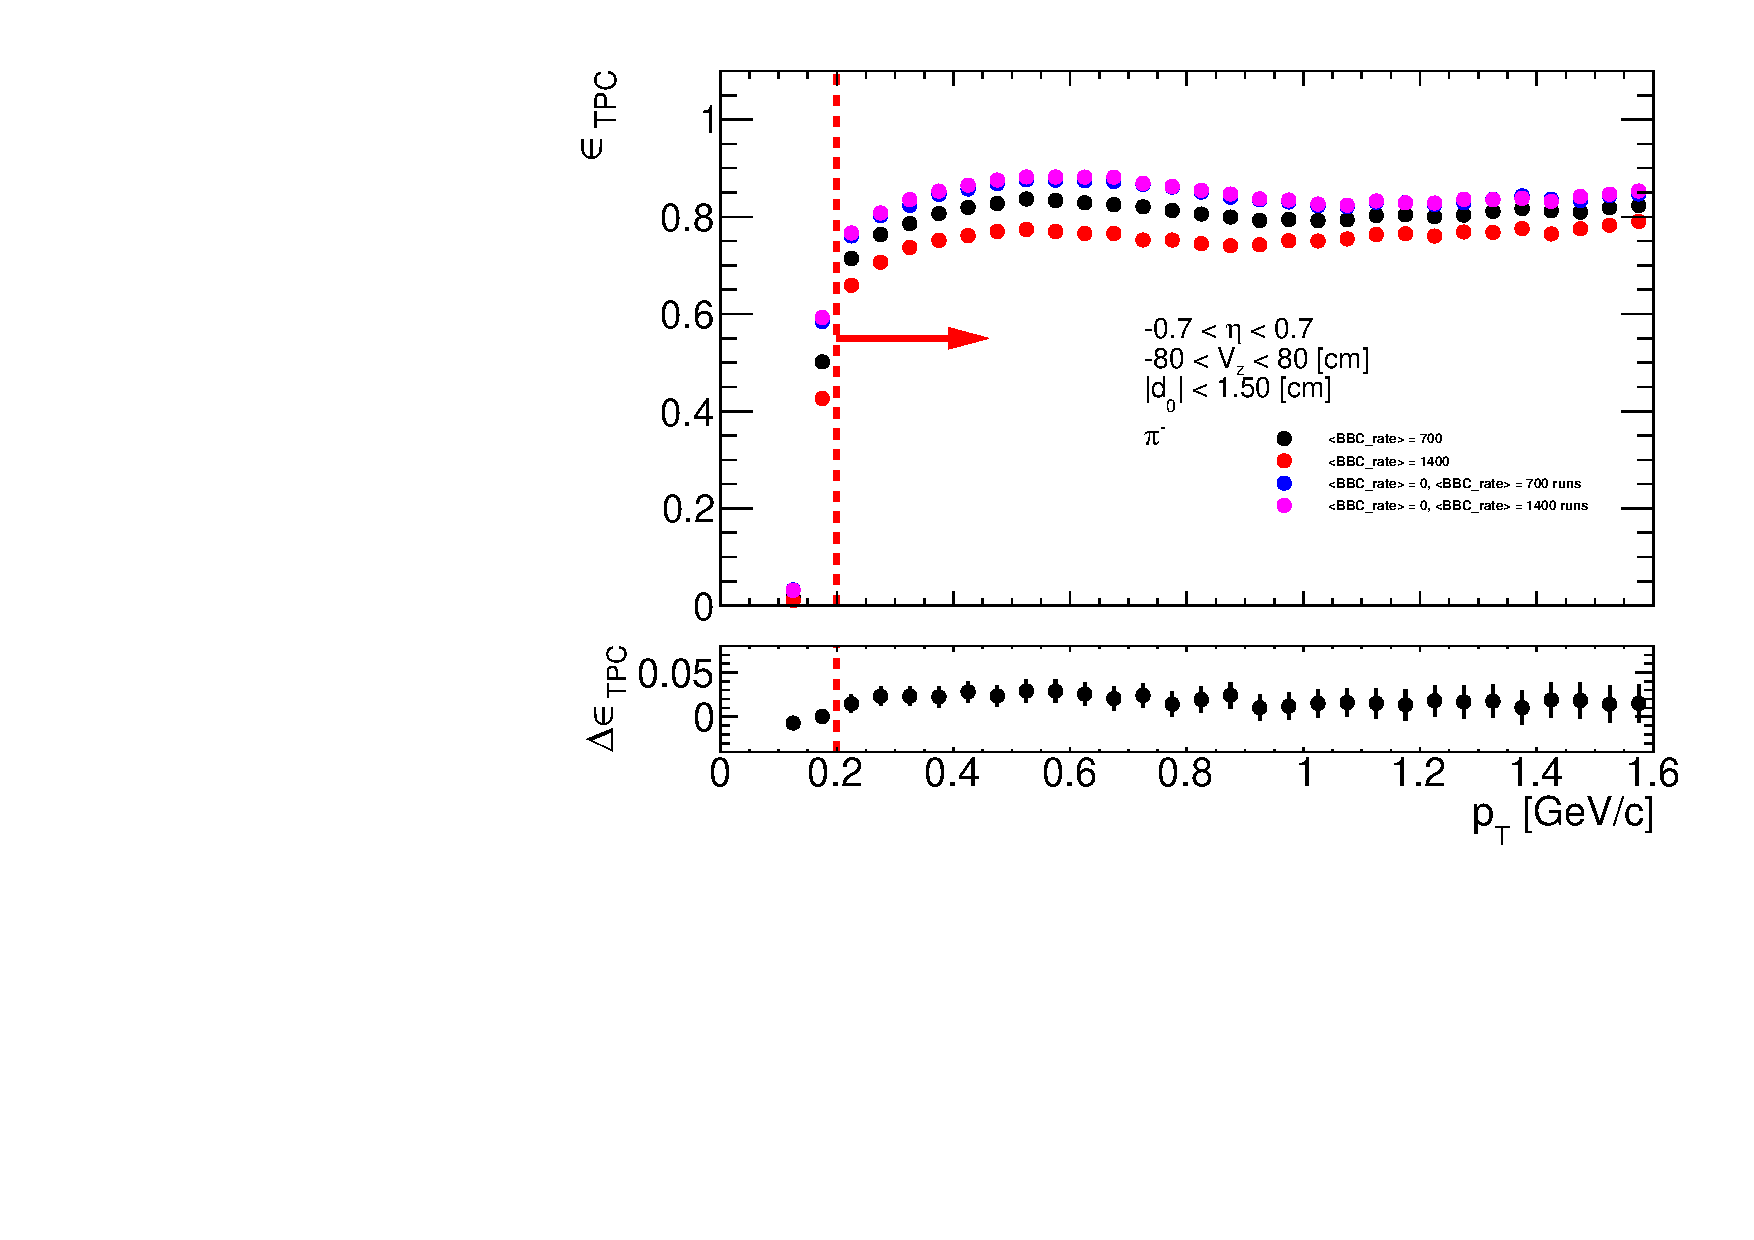
\includegraphics[width=\linewidth,page=1]{graphics/systematicsEfficiency/bbc_and/tpcEffi_d0_1_5_etapt_1.pdf}\\
	}~
	\parbox{0.495\textwidth}{
		\centering
		\includegraphics[width=\linewidth,page=2]{graphics/systematicsEfficiency/bbc_and/tpcEffi_d0_1_5_etapt_1.pdf}\\
	}%
\end{figure}
\begin{figure}[H]
	\caption[The difference $\Delta\epsilon_{ TPC} =\Delta\epsilon_{ TPC}^{1400\text{ kHz}}-2\cdot\Delta\epsilon_{ TPC}^{700\text{ kHz}}$ for $\pi^\pm$ as a function of $p_T$ and $\eta$ $\left(|V_z|<80\text{ cm}\right)$]{The difference $\Delta\epsilon_{ TPC} =\Delta\epsilon_{ TPC}^{1400\text{ kHz}}-2\cdot\Delta\epsilon_{ TPC}^{700\text{ kHz}}$ for $\pi^\pm$ as a function of $p_T$ and $\eta$ $\left(|V_z|<80\text{ cm}\right)$. }
	\label{fig:systError2Dtpc}
	\centering
	\parbox{0.495\textwidth}{
		\centering
		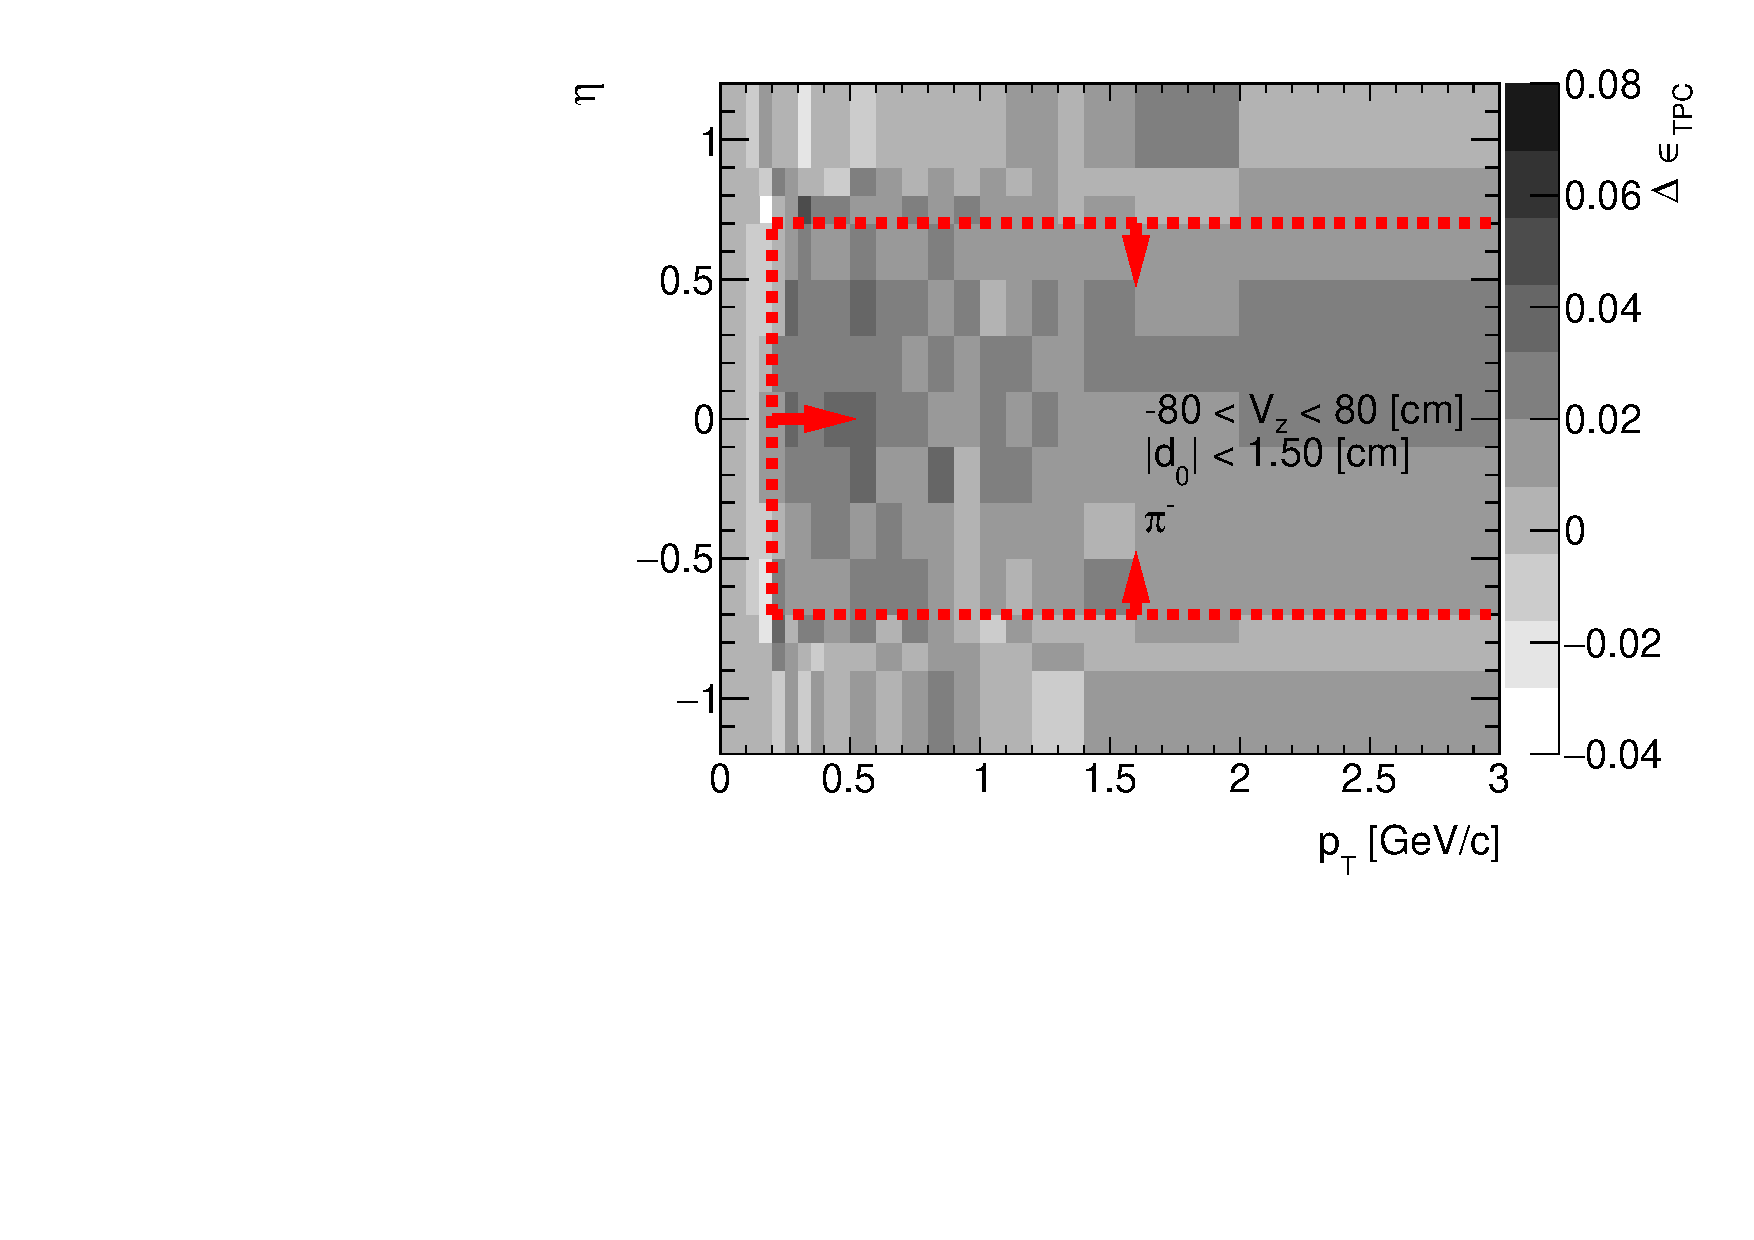
\includegraphics[width=\linewidth,page=1]{graphics/systematicsEfficiency/bbc_and/tpcEffi_d0_1_5_etapt_12D.pdf}\\
	}~
	\parbox{0.495\textwidth}{
		\centering
		\includegraphics[width=\linewidth,page=2]{graphics/systematicsEfficiency/bbc_and/tpcEffi_d0_1_5_etapt_12D.pdf}\\
	}%
\end{figure}

\subsection{Dead material effect on TPC track reconstruction efficiency}\label{sec:deadMaterialSystematics}
The amount of dead material in front of TPC differs up to $20\%$ between data and simulation (see Sec.~\ref{chap:deadMaterial}). First, the~amount of lost particles, $\delta\epsilon_{ TPC}$, due to the interaction with dead material in front of TPC was estimated using  no-pile-up  MC samples. The results for $\pi^-$ in CD are shown in Fig. \ref{fig:dead_materialCD3D}. Then the symmetric systematic uncertainty to the TPC track reconstruction efficiency due to dead material was introduced as $\pm 0.2 \cdot\delta\epsilon_{ TPC}$.
In Fig. \ref{fig:dead_materialCD1D}  the systematic uncertainty is shown for each particle species in CD as a function of $p_T$ $\left(|\eta|<0.7, |V_{z}|<80 \text{ cm}\right)$. 
The results for other particles and SD are shown in Figs. in Appendix \ref{appendix:deadMaterial}.
\begin{figure}[hb]
\caption[The amount of lost $\pi^-$ due to the interaction with dead material in front of TPC as a function of $p_T$, $\eta$ and $z$-vertex in CD]{The amount of lost $\pi^-$ due to the interaction with dead material in front of TPC. Each plot represents the fraction of lost $\pi^-$, $\delta\epsilon_{ TPC}$ ($z$-axis), as a function of true particle pseudorapidity $\eta$ ($y$-axis) and transverse momentum $p_{T}$ ($x$-axis) in single $z$-vertex bin.}\label{fig:dead_materialCD3D}
\centering
\parbox{0.495\textwidth}{
  \centering
  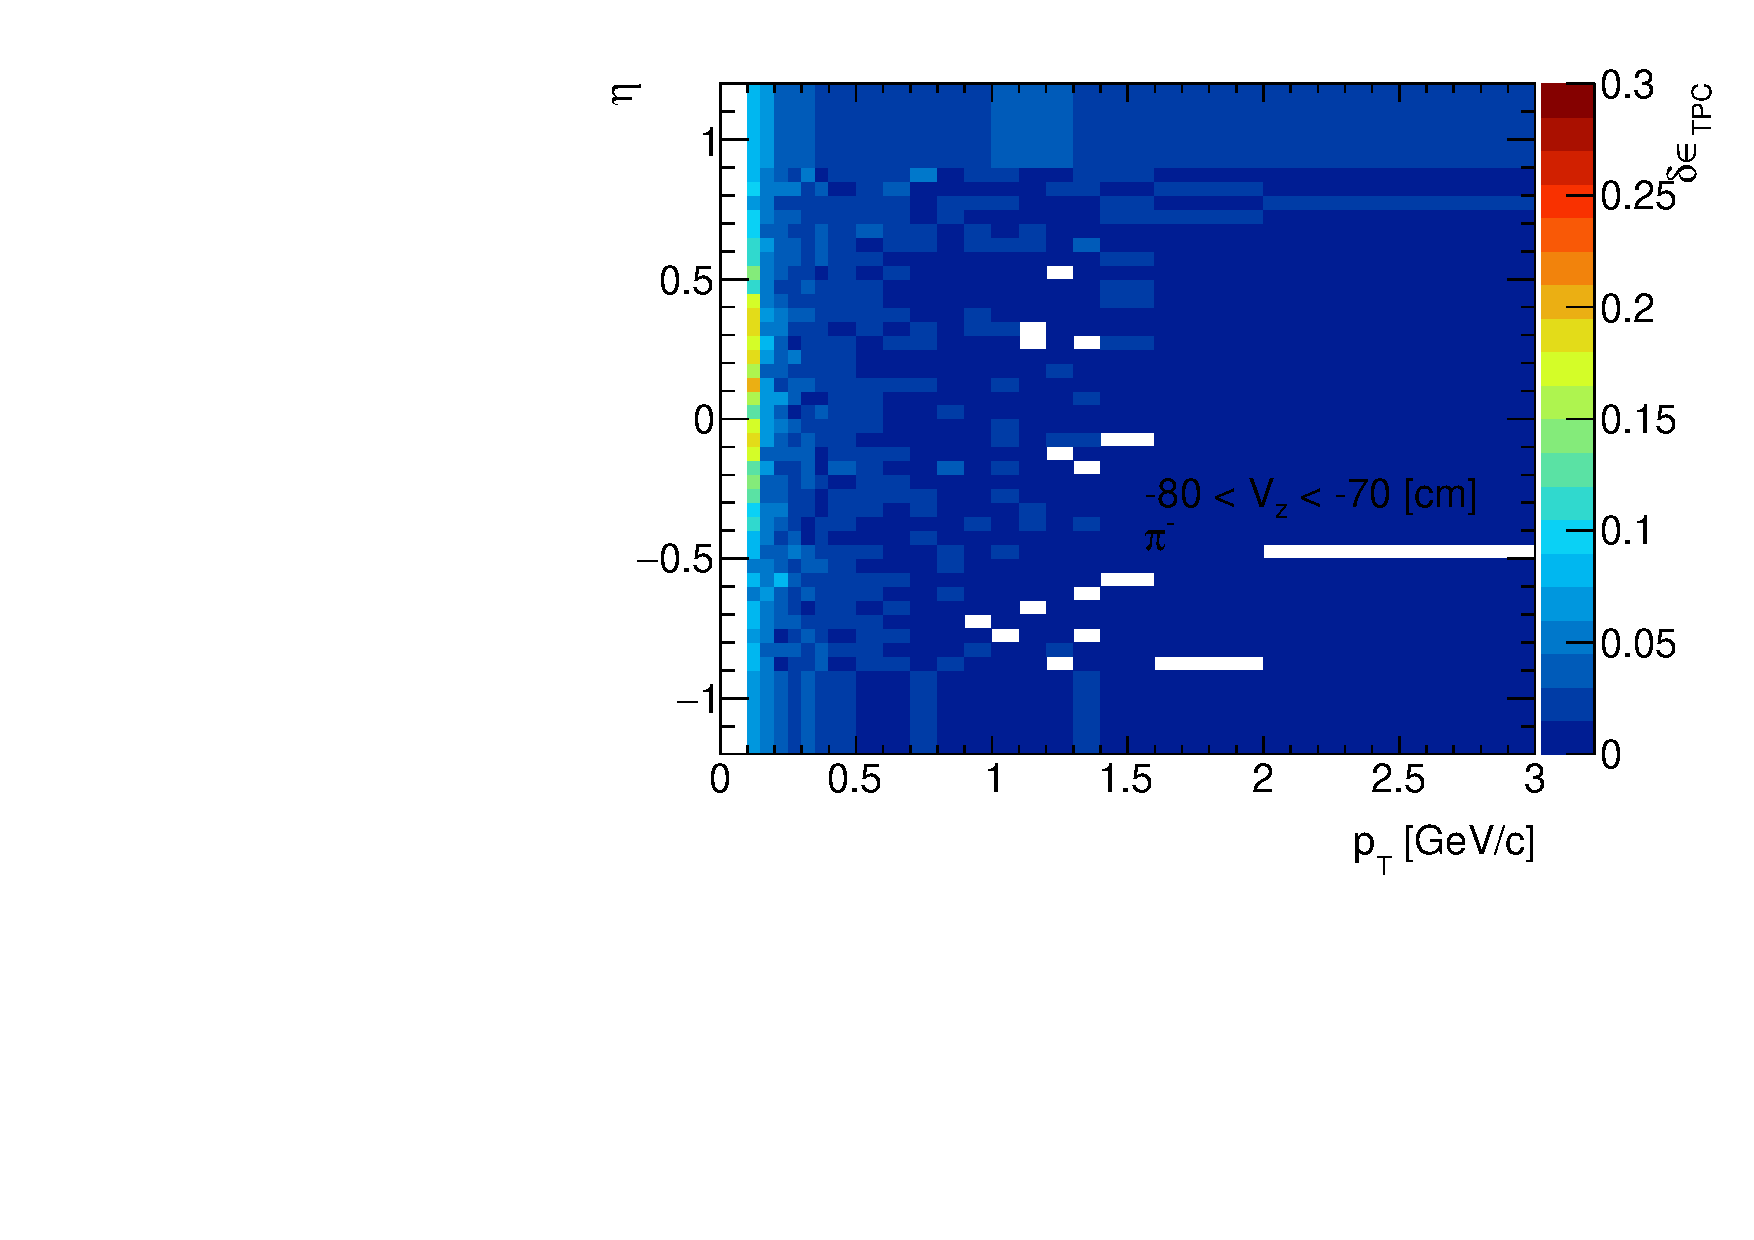
\includegraphics[width=\linewidth,page=1]{graphics/systematicsEfficiency/deadMaterial/secondaries_Unbinned_CD_.pdf}\\
  \includegraphics[width=\linewidth,page=3]{graphics/systematicsEfficiency/deadMaterial/secondaries_Unbinned_CD_.pdf}\\
  \includegraphics[width=\linewidth,page=5]{graphics/systematicsEfficiency/deadMaterial/secondaries_Unbinned_CD_.pdf}\\
  \includegraphics[width=\linewidth,page=7]{graphics/systematicsEfficiency/deadMaterial/secondaries_Unbinned_CD_.pdf}\\
}~
\parbox{0.495\textwidth}{
  \centering
  \includegraphics[width=\linewidth,page=2]{graphics/systematicsEfficiency/deadMaterial/secondaries_Unbinned_CD_.pdf}\\
  \includegraphics[width=\linewidth,page=4]{graphics/systematicsEfficiency/deadMaterial/secondaries_Unbinned_CD_.pdf}\\
  \includegraphics[width=\linewidth,page=6]{graphics/systematicsEfficiency/deadMaterial/secondaries_Unbinned_CD_.pdf}\\
  \includegraphics[width=\linewidth,page=8]{graphics/systematicsEfficiency/deadMaterial/secondaries_Unbinned_CD_.pdf}
}%
\end{figure}
\begin{figure}[hb]\ContinuedFloat
% ~\\[32pt]
\centering
\parbox{0.495\textwidth}{
  \centering
  \includegraphics[width=\linewidth,page=9]{graphics/systematicsEfficiency/deadMaterial/secondaries_Unbinned_CD_.pdf}\\
  \includegraphics[width=\linewidth,page=11]{graphics/systematicsEfficiency/deadMaterial/secondaries_Unbinned_CD_.pdf}\\
  \includegraphics[width=\linewidth,page=13]{graphics/systematicsEfficiency/deadMaterial/secondaries_Unbinned_CD_.pdf}\\
  \includegraphics[width=\linewidth,page=15]{graphics/systematicsEfficiency/deadMaterial/secondaries_Unbinned_CD_.pdf}\\
}~
\parbox{0.495\textwidth}{
  \centering
  \includegraphics[width=\linewidth,page=10]{graphics/systematicsEfficiency/deadMaterial/secondaries_Unbinned_CD_.pdf}\\
  \includegraphics[width=\linewidth,page=12]{graphics/systematicsEfficiency/deadMaterial/secondaries_Unbinned_CD_.pdf}\\
  \includegraphics[width=\linewidth,page=14]{graphics/systematicsEfficiency/deadMaterial/secondaries_Unbinned_CD_.pdf}\\
  \includegraphics[width=\linewidth,page=16]{graphics/systematicsEfficiency/deadMaterial/secondaries_Unbinned_CD_.pdf}
}%
\end{figure}
\begin{figure}[hb]
\caption[The systematic uncertainty to the TPC track reconstruction efficiency due to  amount of dead material in front of TPC using MC samples for CD]{The systematic uncertainty to the TPC track reconstruction efficiency due to  amount of dead material in front of TPC using MC samples for CD. Each plot represents the systematic uncertainty as a~function of true particle $p_T$ $\left(|\eta|<0.7, |V_{z}|<80 \text{ cm}\right)$ for given particle species: $\pi^-$,$\pi^+$, $K^-$, $K^+$, $\bar{p}$ and $p$. It was also calculated for negative and positive particles without identification. }\label{fig:dead_materialCD1D}
\centering
\parbox{0.495\textwidth}{
  \centering
  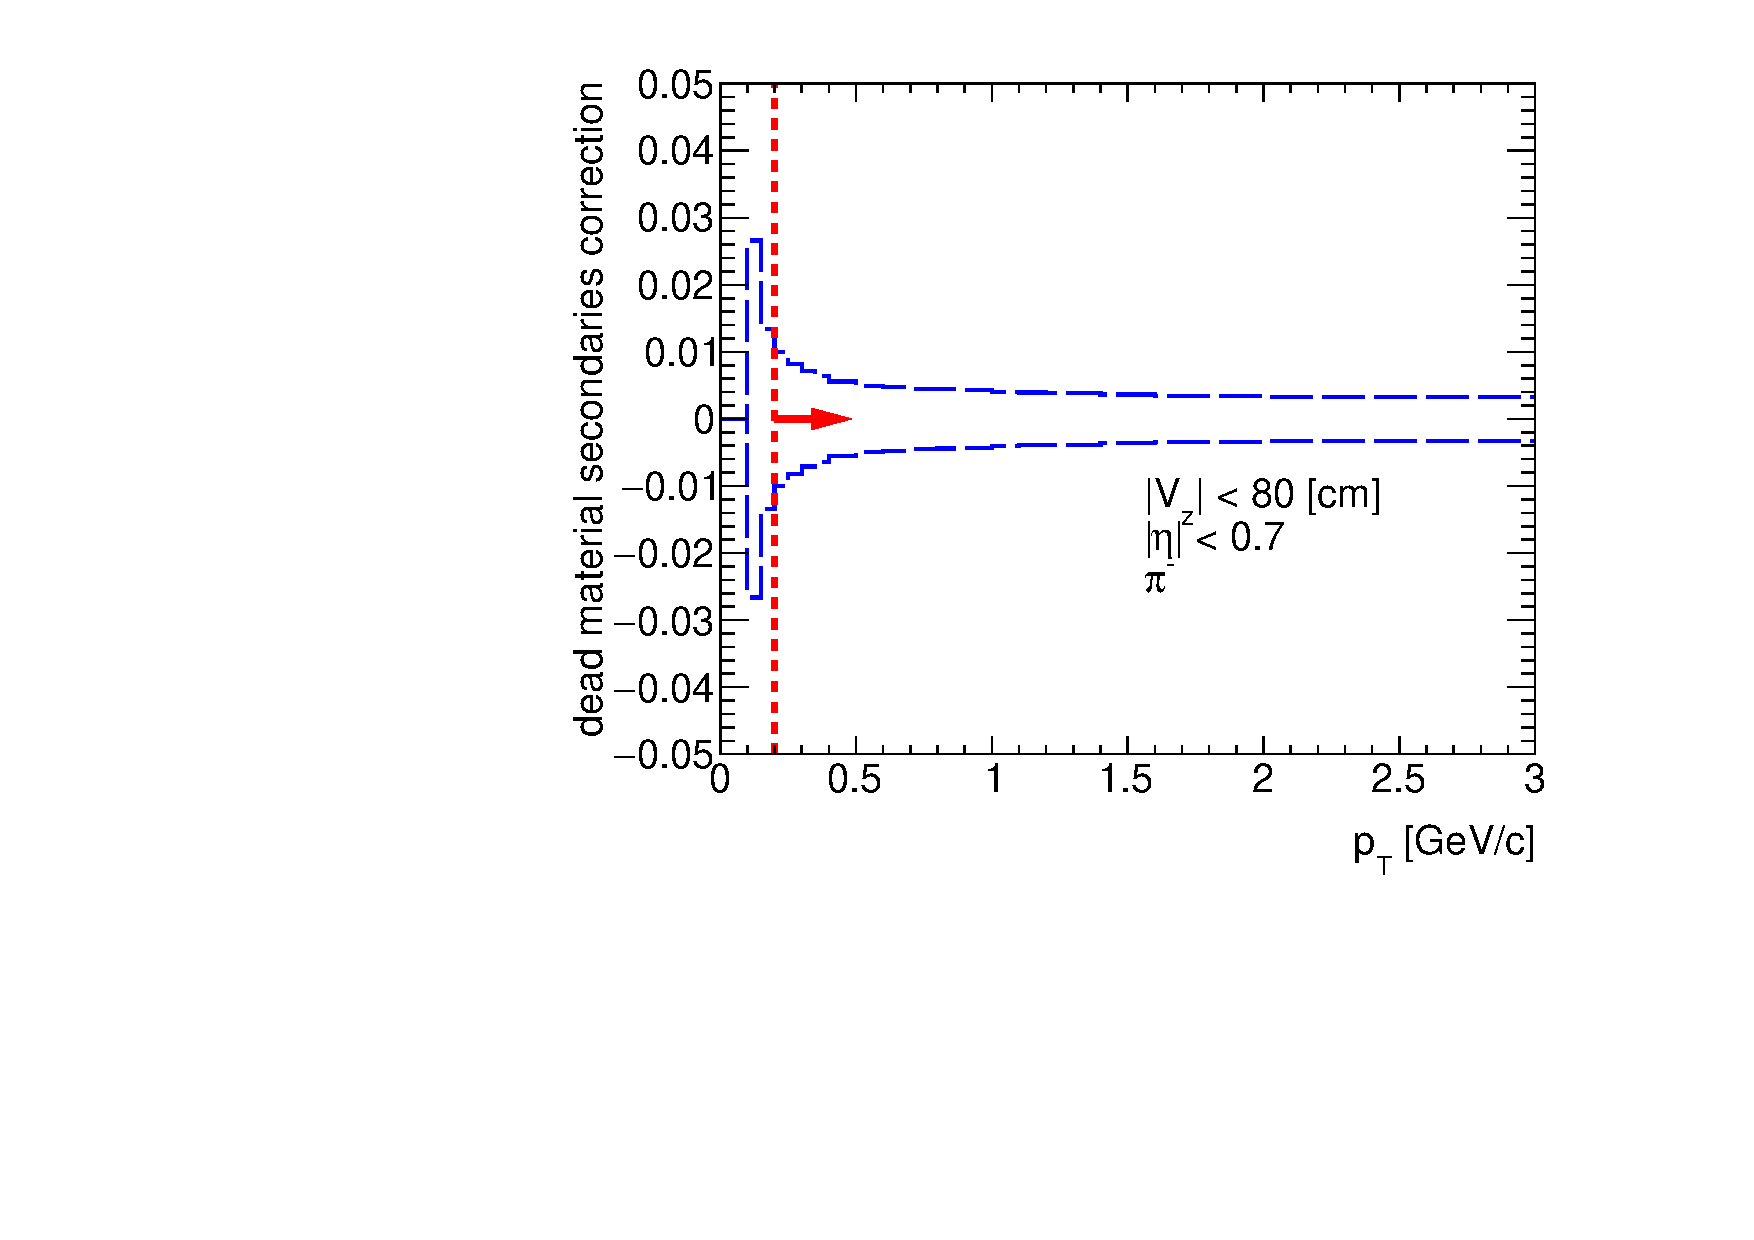
\includegraphics[width=\linewidth,page=1]{graphics/systematicsEfficiency/deadMaterial/secondaries_Unbinned_CD_1D.pdf}\\
  \includegraphics[width=\linewidth,page=2]{graphics/systematicsEfficiency/deadMaterial/secondaries_Unbinned_CD_1D.pdf}\\
  \includegraphics[width=\linewidth,page=3]{graphics/systematicsEfficiency/deadMaterial/secondaries_Unbinned_CD_1D.pdf}\\
  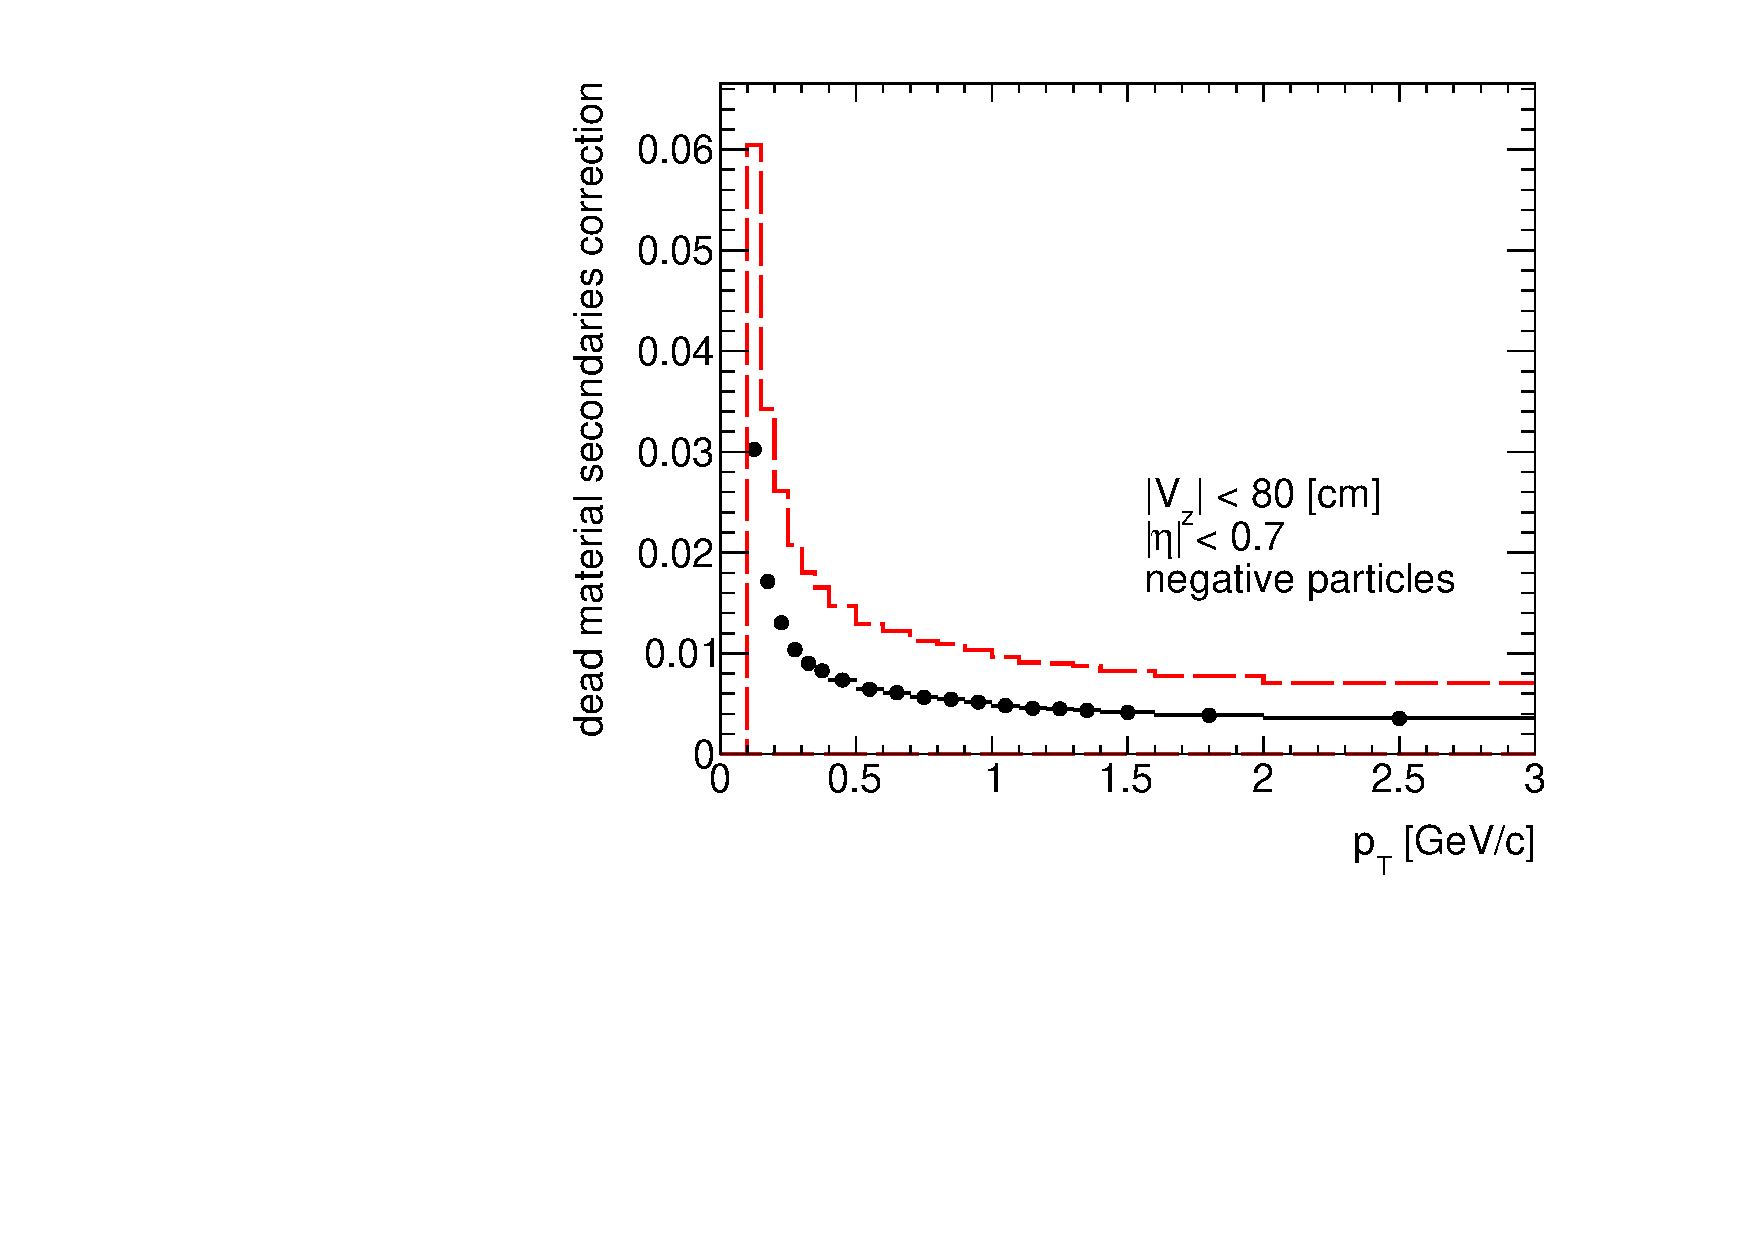
\includegraphics[width=\linewidth,page=1]{graphics/systematicsEfficiency/deadMaterial/secondaries_Unbinned_Charged_CD1D.pdf}\\
}~
\parbox{0.495\textwidth}{
  \centering
  \includegraphics[width=\linewidth,page=4]{graphics/systematicsEfficiency/deadMaterial/secondaries_Unbinned_CD_1D.pdf}\\
  \includegraphics[width=\linewidth,page=5]{graphics/systematicsEfficiency/deadMaterial/secondaries_Unbinned_CD_1D.pdf}\\
  \includegraphics[width=\linewidth,page=6]{graphics/systematicsEfficiency/deadMaterial/secondaries_Unbinned_CD_1D.pdf}\\
  \includegraphics[width=\linewidth,page=2]{graphics/systematicsEfficiency/deadMaterial/secondaries_Unbinned_Charged_CD1D.pdf}
}%
\end{figure}



\section{TOF matching efficiency}\label{sec:tofSystematics}
\subsection{Embedding (pile-up) effect}
The approach to calculate the systematic uncertainty on TOF matching efficiency related to pile-up was quite similar to the one used for TPC track reconstruction efficiency (Sec.~\ref{subsec:TpcEffSystPileUp}). However, the TOF matching efficiency is conditional and depends on TPC track reconstruction efficiency. Since that, the difference between high and low pile-up runs is given by:
\begin{equation}
\Delta\epsilon_{ TOF}^{1400/700\text{ kHz}}=\frac{N_{TPC-TOF}^{no-pile-up}}{N_{TPC}^{no-pile-up}}-\frac{N_{TPC-TOF}^{pile-up}}{N_{TPC}^{pile-up}}
\label{eq:tofSyst}
\end{equation}
where:\\
$N_{TPC-TOF}^{pile-up}$ - number of reconstructed tracks, matched with MC tracks and TOF hit in pile-up MC,\\
$N_{TPC-TOF}^{no-pile-up}$ - number of reconstructed tracks, matched with MC tracks and TOF hit in no-pile-up MC,\\
$N_{TPC}^{pile-up}$ - number of reconstructed tracks, matched with MC tracks in pile-up MC,\\
$N_{TPC}^{no-pile-up}$ - number of reconstructed tracks, matched with MC tracks in no-pile-up MC.

\noindent Next the difference between high and low pile-up events was calculated withe the formula similar to the one given by Eq. \ref{eq:tpcSystDifference} and is shown in \Cref{fig:systError1Dtof,fig:systError2Dtof}. The origin of  $N_{TPC-TOF}$ increase is not known (it may be due to lack of pile-up in TPC or TOF). Since that, it is impossible to correctly calculate the statistical error for $\Delta\epsilon_{ TOF}$. Nevertheless, $\Delta\epsilon_{ TOF}$ is  smaller than $0.5\%$ and can be neglected in comparison with other systematic uncertainties.
\begin{figure}[hb]
	\caption[$\pi^\pm$ TOF matching efficiency as a function of $p_T$ $\left(|\eta|<0.7, |V_z|<80\text{ cm}\right)$ for embedded MC samples with \mbox{$<\text{BBC\_AND}>=700$~kHz} and \mbox{$<\text{BBC\_AND}>=1400$~kHz}]{$\pi^\pm$ TOF matching efficiency as a function of $p_T$ $\left(|\eta|<0.7, |V_z|<80\text{ cm}\right)$ for embedded MC samples with \mbox{$<\text{BBC\_AND}>=700$~kHz} and \mbox{$<\text{BBC\_AND}>=1400$~kHz}. The efficiences from corresponding no-pile-up MC samples were also shown. Additionally, the differences  from Eq. \ref{eq:tpcSystDifference} were drawn in the bottom of each plot.}
	\label{fig:systError1Dtof}
	\centering
	\parbox{0.495\textwidth}{
		\centering
		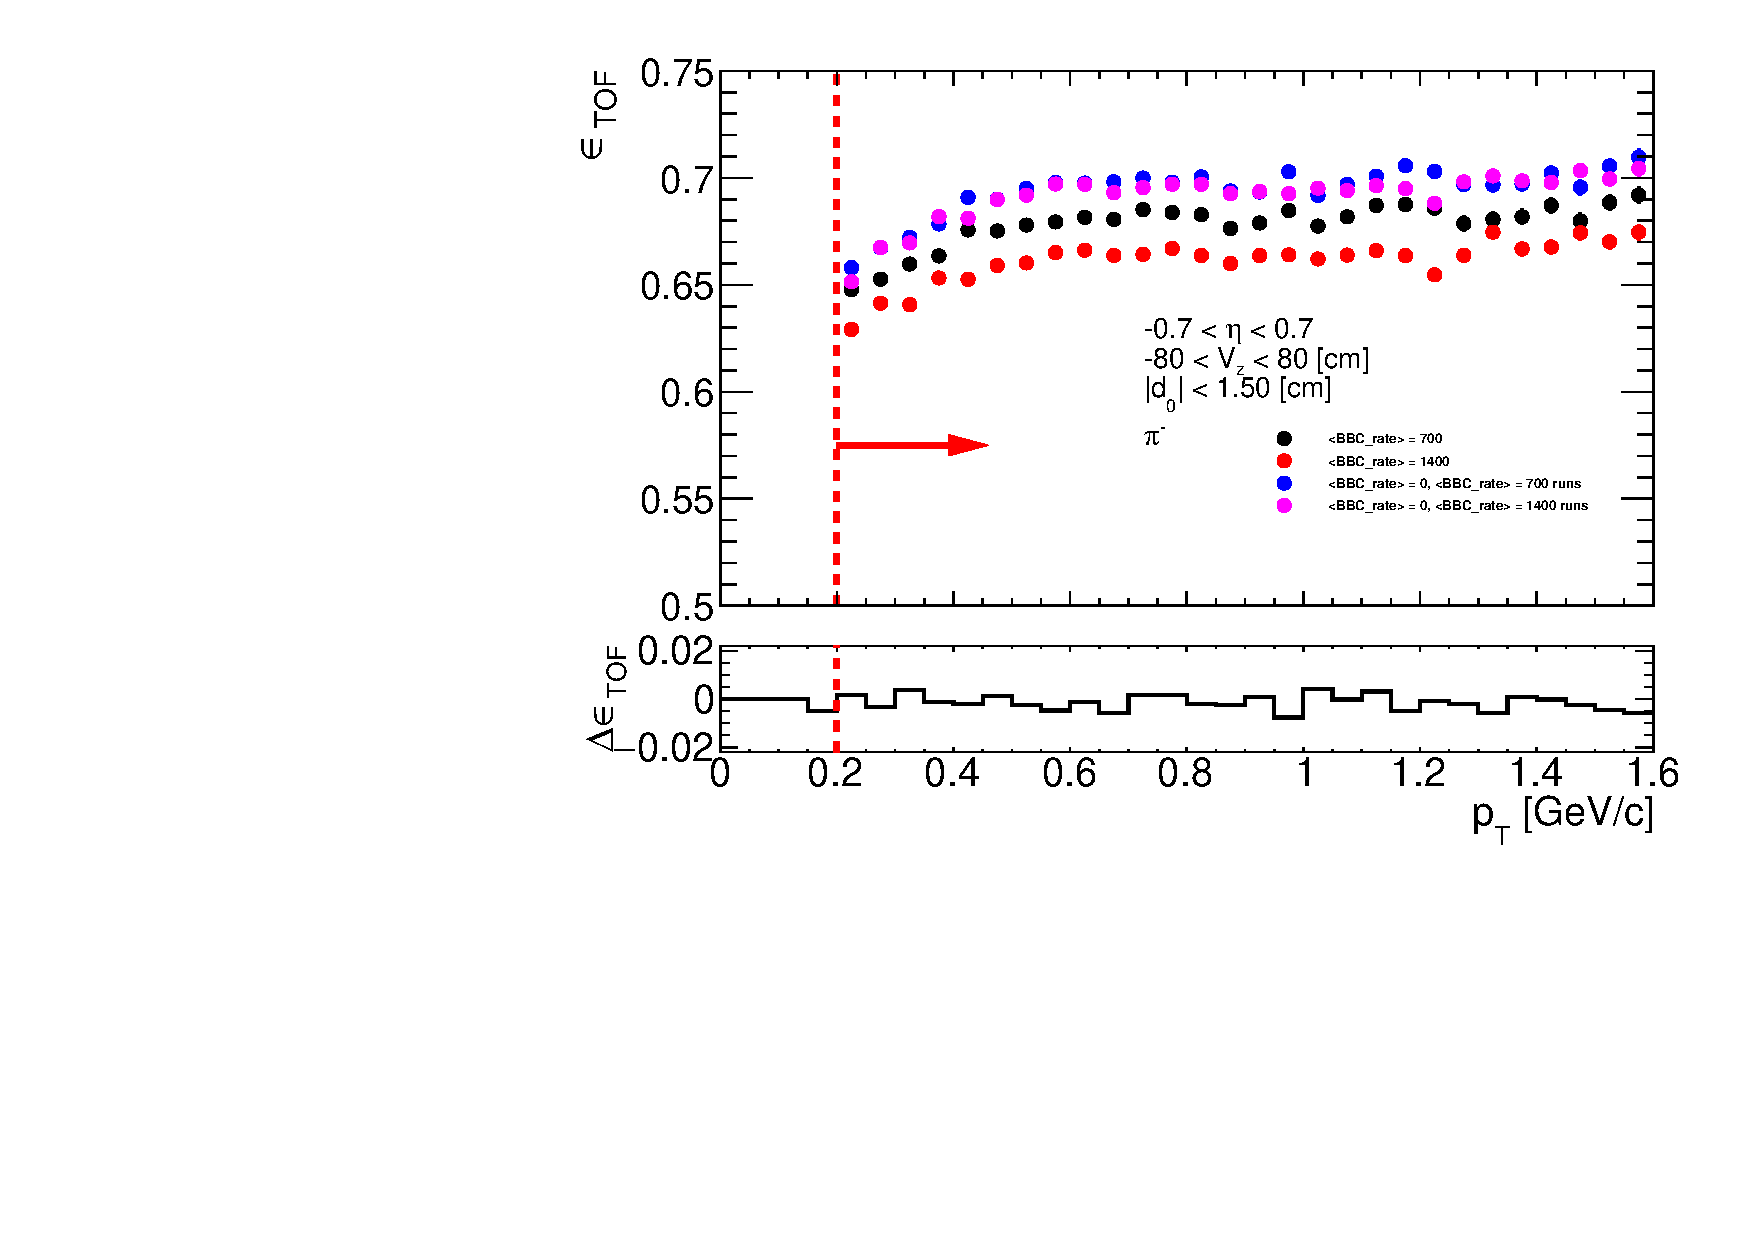
\includegraphics[width=\linewidth,page=1]{graphics/systematicsEfficiency/bbc_and/tofEffi_d0_1_5_etapt_1.pdf}\\
	}~
	\parbox{0.495\textwidth}{
		\centering
		\includegraphics[width=\linewidth,page=2]{graphics/systematicsEfficiency/bbc_and/tofEffi_d0_1_5_etapt_1.pdf}\\
	}%
\end{figure}
\begin{figure}[H]
	\caption[The difference $\Delta\epsilon_{ TOF} =\Delta\epsilon_{ TOF}^{1400\text{ kHz}}-2\cdot\Delta\epsilon_{ TOF}^{700\text{ kHz}}$ for $\pi^\pm$ as a function of $p_T$ and $\eta$ $\left(|V_z|<80\text{ cm}\right)$]{The difference $\Delta\epsilon_{ TOF} =\Delta\epsilon_{ TOF}^{1400\text{ kHz}}-2\cdot\Delta\epsilon_{ TOF}^{700\text{ kHz}}$ for $\pi^\pm$ as a function of $p_T$ and $\eta$ $\left(|V_z|<80\text{ cm}\right)$. }
	\label{fig:systError2Dtof}
	\centering
	\parbox{0.495\textwidth}{
		\centering
		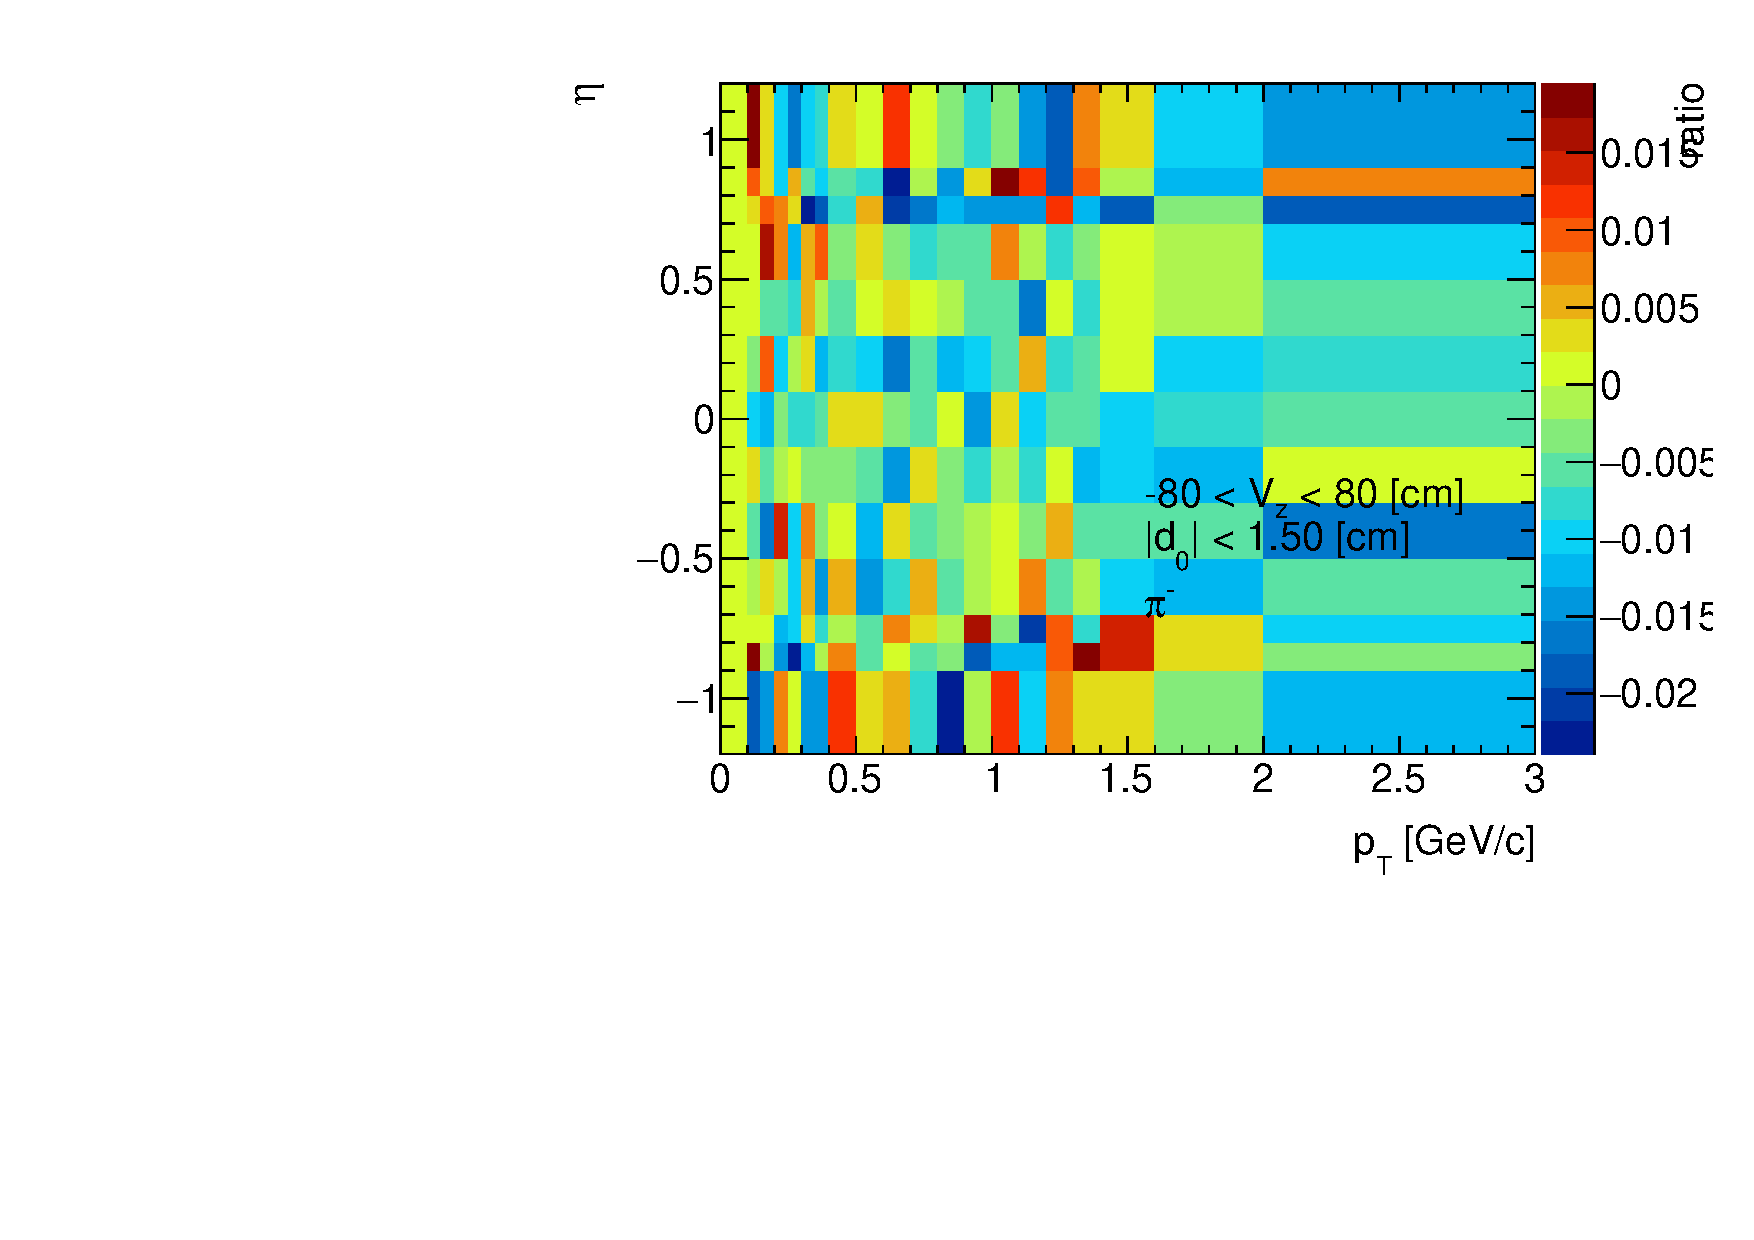
\includegraphics[width=\linewidth,page=1]{graphics/systematicsEfficiency/bbc_and/tofEffi_d0_1_5_etapt_12D.pdf}\\
	}~
	\parbox{0.495\textwidth}{
		\centering
		\includegraphics[width=\linewidth,page=2]{graphics/systematicsEfficiency/bbc_and/tofEffi_d0_1_5_etapt_12D.pdf}\\
	}%
\end{figure}



\subsection{Simulation accuracy (absolute error on TOF efficiency)}\label{subsec:tofAbsEffSystAndCorr}

The efficiency of TOF hit reconstruction and matching with the TPC tracks that was used in our analyses was (at the very beginning) taken directly from the STAR simulation. This made the inaccuracies in the description of real detector geometry and its response propagating to physics results and introducing a bias. We decided to estimate the systematic uncertainty connected with the accuracy of description of the TOF system in (data-embedded) STAR simulation by extracting the TOF efficiency in the very same way from the data and embedded MC and comparing the results. In this section we show the TOF efficiency analysis that led to derivation of the correction to the TOF efficiency and the systematic error of the latter.

Unfortunately, in 2015 there were no low-luminosity (heavy-ion) runs that would imply lack of off-time pile-up tracks in TPC and thus would allow calculating the TOF efficiency in straightforward way, namely by dividing number of selected TPC tracks that were matched with TOF hits by number of all selected TPC tracks (matched or unmatched). For this reason a variation of the ``tag and probe'' method was developed and used. This method utilizes some specific feature of the distribution of quantity describing two objects (whose trigger/reconstriction/identification/etc. efficiency is studied) which allows to quantify amount of these objects with satisfied/unsatisfied efficiency condition. This could be e.g. $J/\psi$ peak in the invariant mass spectrum of the muon tracks, like in the study of muon identification efficiency in MTD~\cite{Huang:2016dbm}. %
%An example could be e.g. extraction of the muon identification efficiency in MTD. The quantity providing characteristic feature would be invariant mass of two opposite-sign tracks, which should contain a $J/\psi$ peak in the invariant mass spectrum for real muon tracks. One could tightly select one track likely being a muon (it would be a tag), and fill the histograms of $m(\mu^{+}\mu^{-})$ for all pairs tag+probe, where probes would be all tracks which 

%---------------------------
\begin{figure}[b!]%\vspace{-2pt}%
\centering%
\begin{minipage}{.4725\textwidth}%
  \centering%\vspace{11pt}
  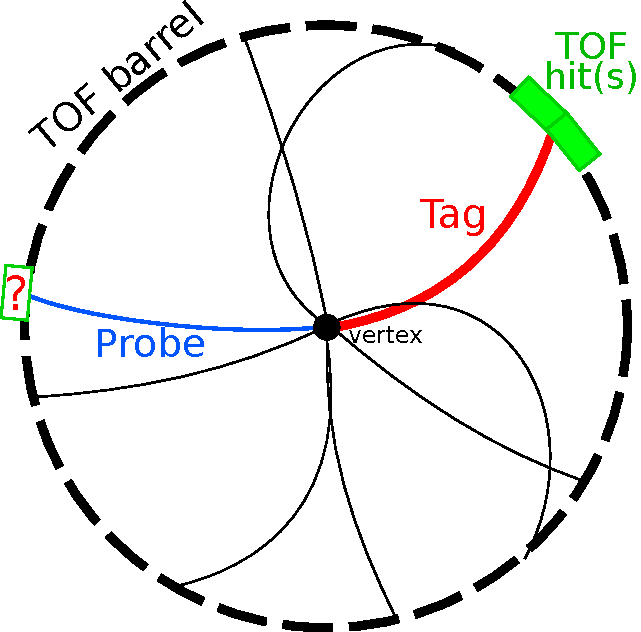
\includegraphics[width=0.98\linewidth]{graphics/systematicsEfficiency/TOF_tagAndProbe/sketch.pdf}%\vspace{-5pt}%
  \caption[Sketch of the tag\&probe method.]%
  {Sketch of the cross section of the central detector and CEP event with off-time pile-up tracks with drafted tag\&probe method used to determine the TOF hit reconstruction and matching efficiency. }\label{fig:tagAndProbeSketch}
\end{minipage}%
\quad\quad%
\begin{minipage}{.4725\textwidth}%
  \centering%
  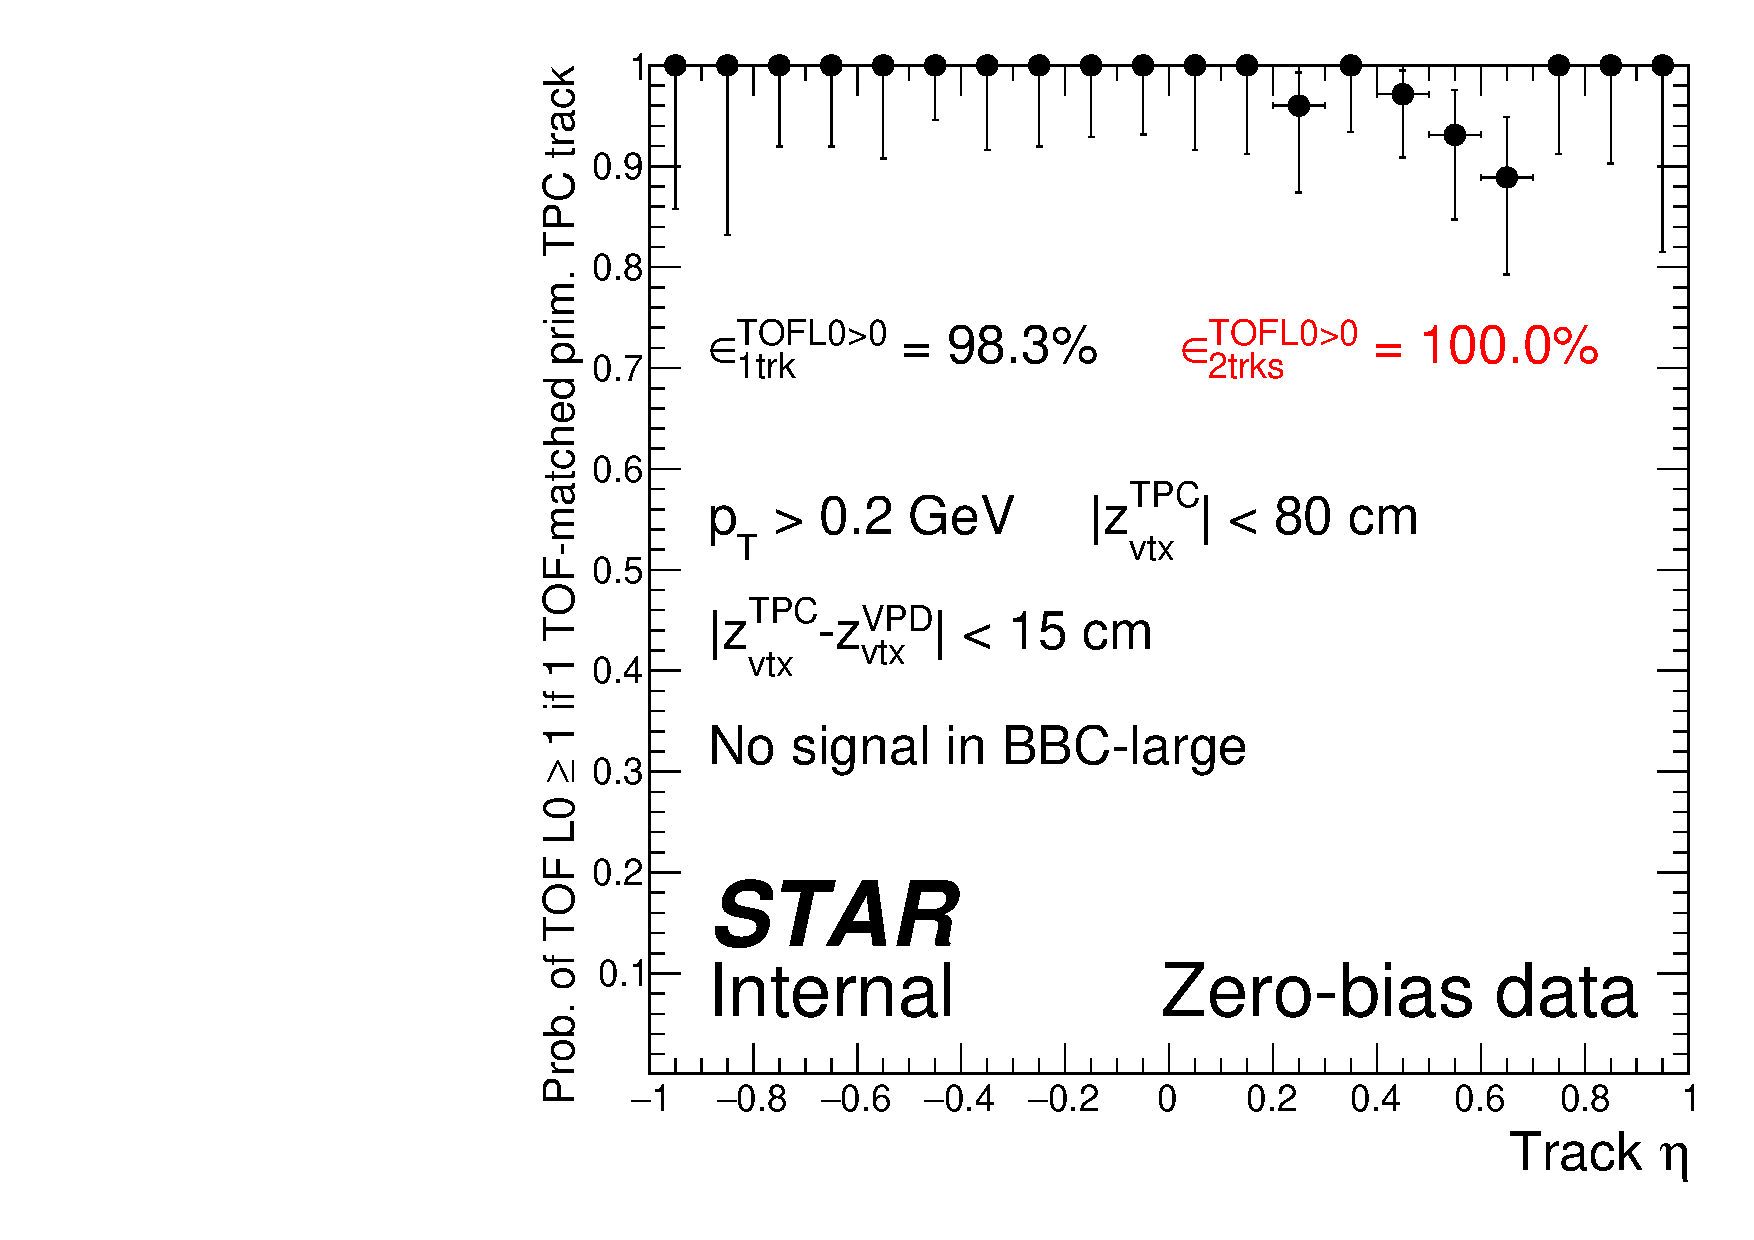
\includegraphics[width=\linewidth]{graphics/systematicsEfficiency/TOF_tagAndProbe/TofL0Eff_1TofVtx_1TofTrack.pdf}%\vspace*{-5pt}
  \caption[Probability of the non-zero TOF L0 multiplicity if 1 primary TOF-matched TPC track vs. track $\eta$.]
   {Probability of the non-zero trigger-level TOF multiplicity in events with exactly 1 primary TPC track matched with offline TOF hit, as a function of track pseudorapidity. VPD signal required.}
   \label{fig:tofTrigEffTagAndProbe}%\vspace*{-29pt}
\end{minipage}%
\end{figure}%
%---------------------------

In our varation of mentioned tag\&probe method the CEP of $\pi^{+}\pi^{-}$ events were used, with the missing transverse momentum $p_{T}^{\text{miss}}$ used to determine signal event yield ($p_{T}^{\text{miss}}=(\vec{p}_{W}+\vec{\pi}^{+}+\vec{\pi}^{-}+\vec{p}_{E})_{T}$). In short, events with forward proton track on each side of STAR and with a TOF-matched primary TPC track (tag) were selected. Among the remaining primary TPC tracks in the same vertex the opposite-sign TPC track (probe) was chosen as the one which provides the minimum total transverse momentum of all four tracks. The probe was checked whether it has been matched with the TOF hit or not. The ratio of the matched TPC tracks to all (matched or unmatched) TPC tracks defined the TOF efficiency, as given in Eq.~\eqref{eq:tagAndProbeEffDef}:%
\begin{equation}\label{eq:tagAndProbeEffDef}%
\varepsilon^{\text{TOF}}=\frac{N^{\text{probes}}_{\text{satisified}}}{N^{\text{probes}}_{\text{produced}}} = \frac{\textcolor{dgreen}{N^{\text{probes}}_{\text{satisified}}}}{\textcolor{dgreen}{N^{\text{probes}}_{\text{satisified}}}+\textcolor{red}{N^{\text{probes}}_{\text{failed}}}} = \frac{\textcolor{dgreen}{2 N^{\text{events}}_{TT}} + \textcolor{dgreen}{N^{\text{events}}_{TP_{s}}}}{\textcolor{dgreen}{2 N^{\text{events}}_{TT}} + \textcolor{dgreen}{N^{\text{events}}_{TP_{s}}} + \textcolor{red}{N^{\text{events}}_{TP_{f}}}}
\end{equation}%
Subscripts $TT$, $TP_{s}$ and $TP_{f}$ denote possible combinations of tags and probes:\\[-17pt]
\begin{itemize}%\scriptsize
 \item $TT$ (both objects satisfy tag criteria, and by definition the efficiency condition); such events provide two probes which satisfy efficiency condition which is the reason for the factor '2' in front of $N^{\text{events}}_{TT}$ in Eq.~\eqref{eq:tagAndProbeEffDef},\\[-17pt]
 \item $TP_{s}$ (one is tag, the other is a probe and probe satisifes the efficiency condition),\\[-17pt]
 \item $TP_{f}$ (one is tag, the other is a probe and probe fails to satisify the eff. condition).%\\[-7pt]
\end{itemize}%
The method is illustrated in the sketch in Fig.~\ref{fig:tagAndProbeSketch}. The detailed description of the procedure of the TOF efficiency extraction is provided in the next page.\newpage

% \[\varepsilon^{\text{TOF}}=\frac{ \textcolor{dgreen}{N^{\text{matched}}_\text{weighted}} }{ N^{\text{all}}_\text{weighted}} = \frac{ \textcolor{dgreen}{N^{\text{matched}}_\text{weighted}} }{ \textcolor{dgreen}{N^{\text{matched}}_\text{weighted}} + \textcolor{red}{N^{\text{not matched}}_\text{weighted}} }\]

The algorithm of tag\&probe method:
\begin{enumerate}
 \item Data from RP\_CPT trigger was used. This trigger required at least a single level-0 TOF hit (trigger details can be found in Tab.~2.1 of Ref.~\cite{AnalysisNoteRafal}). Embedded $\pi^{+}\pi^{-}$ GenEx MC sample was subjected to the same trigger conditions. Since there is no simulation of the TOF trigger we assumed in MC analysis that any reconstructed offline TOF hit guarantees the L0 TOF multiplicity $\geq0$. In Fig.~\ref{fig:tofTrigEffTagAndProbe} we show that this assumption is safe. Appropriate correction is applied in the event weighting procedure, as explained later.\\[-16pt]% in the text.
 \item Events were selected with the following set of cuts from nominal CEP analysis (Ref.~\cite{AnalysisNoteRafal}): \textbf{C1}, \textbf{C2} (TPC vertex), \textbf{C4} (RP tracks), \textbf{C5} (TPC-RP vertex matching), \textbf{C6} (veto signal in large BBC), providing significant reduction of background events.\\[-16pt]
 \item For each event passing above selection primary TOF-matched TPC tracks of good quality (satisfying cuts~\ref{sec:TpcQualityCuts},\ref{sec:TpcDcaCuts}) and compatible with pion hypothesis based on $dE/dx$ ($|n^{\sigma}_{\text{pion}}|<3$) were selected. If any TOF-matched track incompatible with pion hypothesis was found, event was dropped from further analysis. Also, an event was not analyzed if more than 2 TOF-matched tracks were reconstructed (not CEP event).\\[-16pt]
 \item Among primary TOF-matched TPC tracks preselected in \#3, one was set as a tag. In case only one track passed preselection, steps \#5-\#6 were executed only with this single track being a tag. Otherwise steps \#5-\#6 were repeated for every preselected track set as a tag.\\[-16pt]
 \item From the remaining TPC tracks in the same vertex of the sign opposite to tag and of good quality (cuts~\ref{sec:TpcQualityCuts},\ref{sec:TpcDcaCuts}), the one which provided the best transverse momentum balance together with 2 protons and a tag was selected as probe (signature of exclusive $\pi^{+}\pi^{-}$:  $p_{T}^{\text{miss}}\sim0$). If no primary TPC tracks passing this selection were found, an event was dropped.\\[-16pt]
 \item 2-dimensional histograms of quantities of interest (probe $\eta$, probe $p_{T}$) vs. $p_{T}^{\text{miss}}$ were filled, separately for all probes and only for probes matched with TOF. Each probe was associated with the weight $w$ taking into account the trigger efficiency and vertexing efficiency, as given in Eq.~\eqref{eq:tagAndProbeWeigth} and explained later in the text.\\[-16pt]
 \item In each bin of quantity of interest $q$ (as a function of which the efficiency was to be determined) the distribution of $p_{T}^{\text{miss}}$ was fitted  in the signal-free with the function describing background shape. The background was extrapolated to $p_{T}^{\text{miss}}=0$. The signal yield in given bin of $q$ was calculated as the integral of the histogram with subtracted integral of the background function, both in the range $p_{T}^{\text{miss}}<75$~MeV. The final efficiency in given bin of $q$ was calculated according to Eq.~\eqref{eq:tagAndProbeEffDef2}:
 \begin{equation}\label{eq:tagAndProbeEffDef2}
  \varepsilon^{\text{TOF}}(q) = \frac{N_\text{weighted}^{\text{matched},~p_{T}^{\text{miss}}<75~\text{MeV}} - N_\text{bkgd,weighted}^{\text{matched},~p_{T}^{\text{miss}}<75~\text{MeV}} }{ N_\text{weighted}^{\text{all},~p_{T}^{\text{miss}}<75~\text{MeV}} - N_\text{bkgd,weighted}^{\text{all},~p_{T}^{\text{miss}}<75~\text{MeV}} }\vspace*{-25pt}
 \end{equation}

\end{enumerate}

%---------------------------
\begin{figure}[b!]\vspace*{-25pt}
\centering
\parbox{0.4725\textwidth}{
  \centering
  \begin{subfigure}[b]{\linewidth}{
                \subcaptionbox{\label{fig:sampleMissingPtTagAndProbe_DATA}}{\includegraphics[width=\linewidth,page=7]{graphics/systematicsEfficiency/TOF_tagAndProbe/Fitting_effVsPt_data.pdf}\vspace{-10pt}}}
  \end{subfigure}
}
\quad
\parbox{0.4725\textwidth}{
  \centering
    \begin{subfigure}[b]{\linewidth}{
                \subcaptionbox{\label{fig:sampleMissingPtTagAndProbe_MC}}{\includegraphics[width=\linewidth,page=7]{graphics/systematicsEfficiency/TOF_tagAndProbe/Fitting_effVsPt_mc.pdf}\vspace{-10pt}}}
  \end{subfigure}
}%\vspace{-5pt}%
\caption[Sample distributions of $p_{T}^{\text{miss}}$ of the $p$+Tag+Probe+$p$ system in the data and embedded MC.]%
    {Sample distributions of total transverse momentum $p_{T}^{\text{miss}}$ of the $p$+Tag+Probe+$p$ system in the data (\ref{fig:sampleMissingPtTagAndProbe_DATA}) and signal+background embedded MC (\ref{fig:sampleMissingPtTagAndProbe_MC}). TOF-matched and all (matched or unmatched) probes are represented by histograms in green and black color, respectively. The red dashed line shows the exclusivity cut value ($75~\text{MeV}/c$). Signal yield is determined via the integral of the histogram with subtracted integral of the solid line representing non-exclusive background in the $p_{T}^{\text{miss}}$ range to the left from the vertical line. Background (solid line) is fitted with 2$^{\text{nd}}$ order polynomial in the signal-free region (the details can be found in Ref.~\cite{AnalysisNoteRafal} in Sec.~5.2). Full sets of histograms in different ranges of probe $p_{T}$ and $\eta$ are included in Appendix~\ref{appendix:tagAndProbeTofEff}.}\label{fig:sampleMissingPtTagAndProbe}%
\end{figure}
%---------------------------


\newpage


ttt

\begin{equation}\label{eq:tagAndProbeWeigth}%
w=\left\{
\begin{array}{ll}
\left(\epsilon^{\text{TOFL0}>0}_{1\text{trk}}\right)^{-1}~\times~\left(\varepsilon_{vtx}^{\text{nTOF=2}}(\Delta z_{0})\right)^{-1} & \textrm{for~}TT,~TP_{s}\\
\left(\epsilon^{\text{TOFL0}>0}_{2\text{trks}}\right)^{-1}~\times~\left(\varepsilon_{vtx}^{\text{nTOF=1}}(d_{0})\times \varepsilon_{vtx}^{\text{no-TOF}}(\text{DCA}_{z},\text{DCA}_{R})\right)^{-1} & \textrm{for~}TP_{f}
\end{array}
\right.
\end{equation}
 
 
%---------------------------
\begin{figure}[b!]
\centering
\parbox{0.4725\textwidth}{
  \centering
  \begin{subfigure}[b]{\linewidth}
                \subcaptionbox{\label{fig:vertexingEffVsD0}}{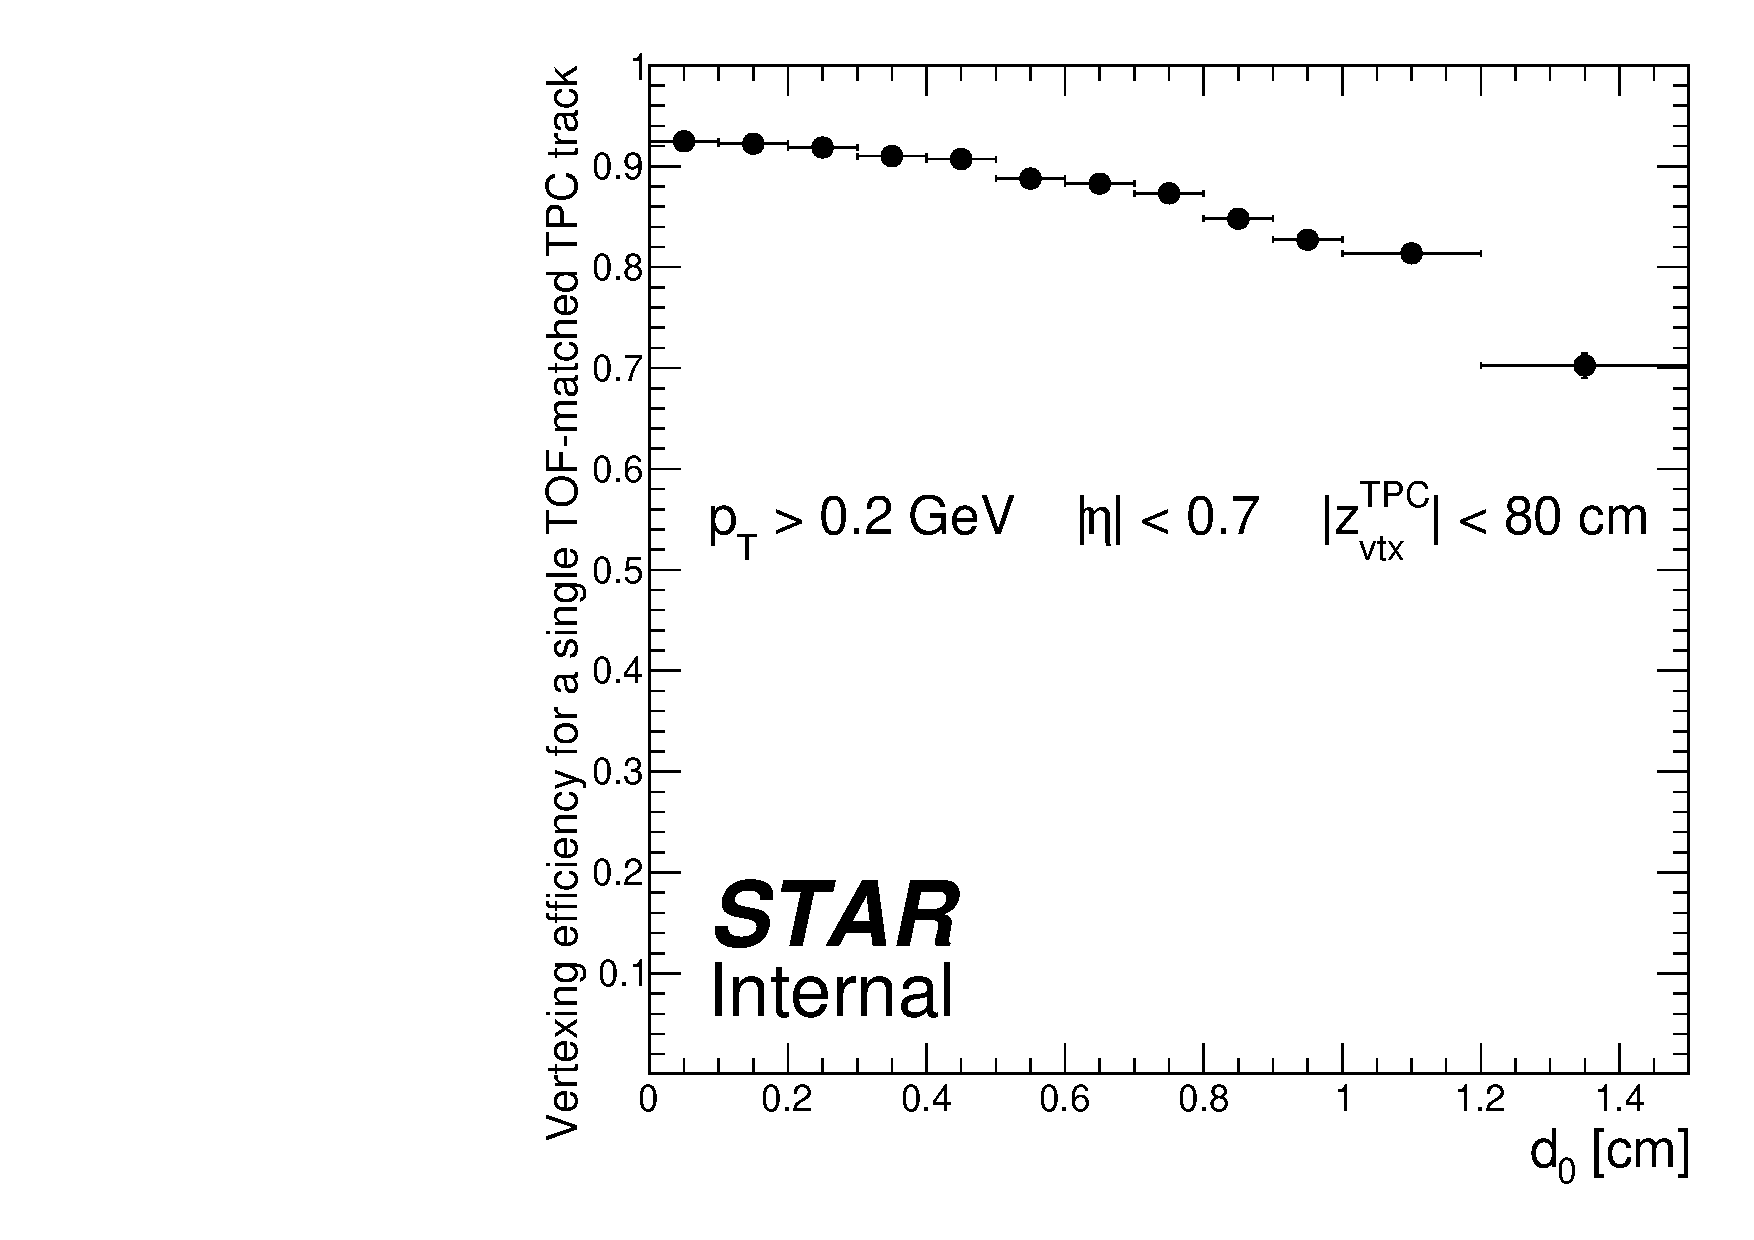
\includegraphics[width=\linewidth]{graphics/systematicsEfficiency/TOF_tagAndProbe/VertexingEffVsD0.pdf}}\vspace{-5pt}
  \end{subfigure}
}%
\quad\quad%
\parbox{0.4725\textwidth}{
  \centering
  \begin{subfigure}[b]{\linewidth}
                \subcaptionbox{\label{fig:vertexingEff2D}}{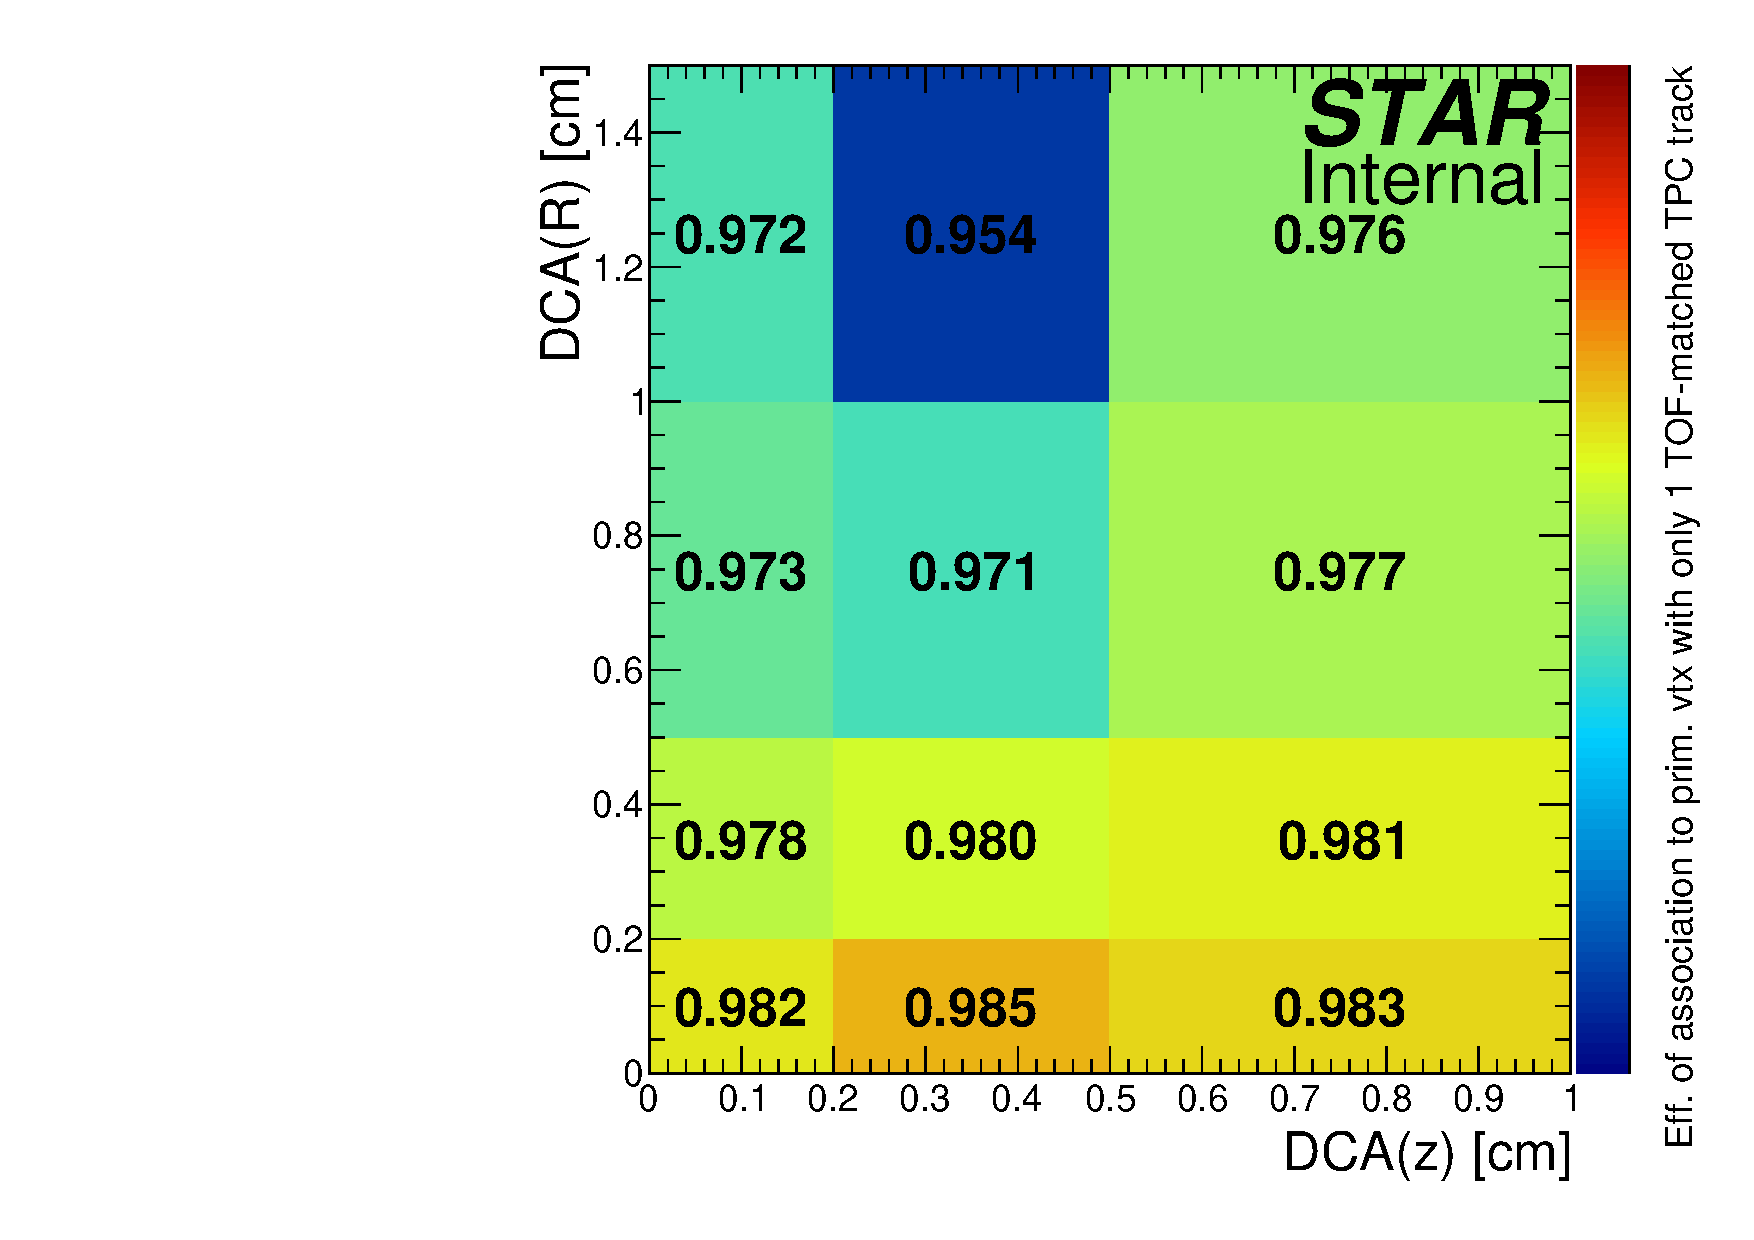
\includegraphics[width=\linewidth]{graphics/systematicsEfficiency/TOF_tagAndProbe/VertexingEffVsDCA_2D.pdf}}\vspace{-5pt}
  \end{subfigure}
}%
\caption[Efficiencies for reconstruction of the vertex with single TOF-matched TPC track and association with this vertex of TOF-unmatched track.]%
    {Efficiency $\varepsilon_{vtx}^{\text{nTOF=1}}$ of reconstruction of the primary vertex from a single TOF-matched TPC track as a function of the transverse impact parameter $d_{0}$ (\ref{fig:vertexingEffVsD0}) and efficiency $\varepsilon_{vtx}^{\text{no-TOF}}$ of association with the vertex formed from single TOF-matched track of a TPC track not matched with TOF, as a function of radial and longitudinal DCA to the vertex (\ref{fig:vertexingEff2D}). The tracks were required to be matched with true-level primary particles (pions) as well as the quality and kinematic cuts were implied (\ref{sec:TpcQualityCuts}, \ref{sec:TpcDcaCuts}, \ref{sec:TpcKinematicCuts}).}\label{fig:vertexingEffTagAndProbe}%
\end{figure}
%---------------------------

% \begin{equation}\label{eq:tofEffFunc}
%  \varepsilon^{\text{TOF}}(p_{T}) = A\cdot \exp\Big\{-\left(B/p_{T}\right)^{C}\Big\}
% \end{equation}

% \begin{equation}\label{eq:nProbeTof}
%  n_{\text{probe}}^{\text{TOF}}~=~\underbrace{N\times\varepsilon^{\text{TOF}}\varepsilon_{\text{vtx}}^{\bis}\times\varepsilon^{\text{TOF}}}_{\pi^{+}~\text{is tag},~\pi^{-}~\text{is probe}}~+~\underbrace{N\times\varepsilon^{\text{TOF}}\times\varepsilon^{\text{TOF}}\varepsilon_{\text{vtx}}^{\bis}}_{\pi^{+}~\text{is probe},~\pi^{-}~\text{is tag}}~=~ 2N\left(\varepsilon^{\text{TOF}}\right)^{2}\varepsilon_{\text{vtx}}^{\bis}
% \end{equation}


% \begin{equation}\label{eq:nProbeNoTof}
%  n_{\text{probe}}^{!\text{TOF}}~=~\underbrace{N\times\varepsilon^{\text{TOF}}\varepsilon_{\text{vtx}}^{\prime}\times\left(1-\varepsilon^{\text{TOF}}\right)}_{\pi^{+}~\text{is tag},~\pi^{-}~\text{is probe}}~+~\underbrace{N\times\left(1-\varepsilon^{\text{TOF}}\right)\times\varepsilon^{\text{TOF}}\varepsilon_{\text{vtx}}^{\prime}}_{\pi^{+}~\text{is probe},~\pi^{-}~\text{is tag}}~=~ 2N\left(1-\varepsilon^{\text{TOF}}\right)\varepsilon^{\text{TOF}}\varepsilon_{\text{vtx}}^{\prime}
% \end{equation}


% \begin{multicols}{3}%~\\[-30pt]
% \begin{equation}\label{eq:nProbeTofTilde}
%  \tilde{n}_{\text{probe}}^{\text{TOF}}~=~\frac{n_{\text{probe}}^{\text{TOF}}}{\varepsilon_{\text{vtx}}^{\bis}}
% \end{equation}
%    \break\\[-20pt]
%     \begin{equation}\label{eq:nProbeNoTofTilde}
%  \tilde{n}_{\text{probe}}^{!\text{TOF}}~=~\frac{n_{\text{probe}}^{!\text{TOF}}}{\varepsilon_{\text{vtx}}^{\prime}}
% \end{equation}
% \break\\[-20pt]
% \begin{equation}\label{eq:tofEffTagAndProbe}
%  \varepsilon^{\text{TOF}} = \frac{\tilde{n}_{\text{probe}}^{\text{TOF}}}{\tilde{n}_{\text{probe}}^{\text{TOF}}~+~\tilde{n}_{\text{probe}}^{!\text{TOF}}}
% \end{equation}
%     \end{multicols}
    
% \begin{equation}\label{eq:nProbeTofTilde}
%  \tilde{n}_{\text{probe}}^{\text{TOF}}~=~\frac{n_{\text{probe}}^{\text{TOF}}}{\varepsilon_{\text{vtx}}^{\bis}}
% \end{equation}
% 
% 
% \begin{equation}\label{eq:nProbeNoTofTilde}
%  \tilde{n}_{\text{probe}}^{!\text{TOF}}~=~\frac{n_{\text{probe}}^{!\text{TOF}}}{\varepsilon_{\text{vtx}}^{\prime}}
% \end{equation}
% 
% \begin{equation}\label{eq:tofEffTagAndProbe}
%  \varepsilon^{\text{TOF}} = \frac{\tilde{n}_{\text{probe}}^{\text{TOF}}}{\tilde{n}_{\text{probe}}^{\text{TOF}}~+~\tilde{n}_{\text{probe}}^{!\text{TOF}}}
% \end{equation}








%---------------------------
\begin{figure}[h!]
\centering
\parbox{0.4725\textwidth}{
  \centering
  \begin{subfigure}[b]{\linewidth}{
                \subcaptionbox{\label{fig:tofEffSystVsPt_CPT}}{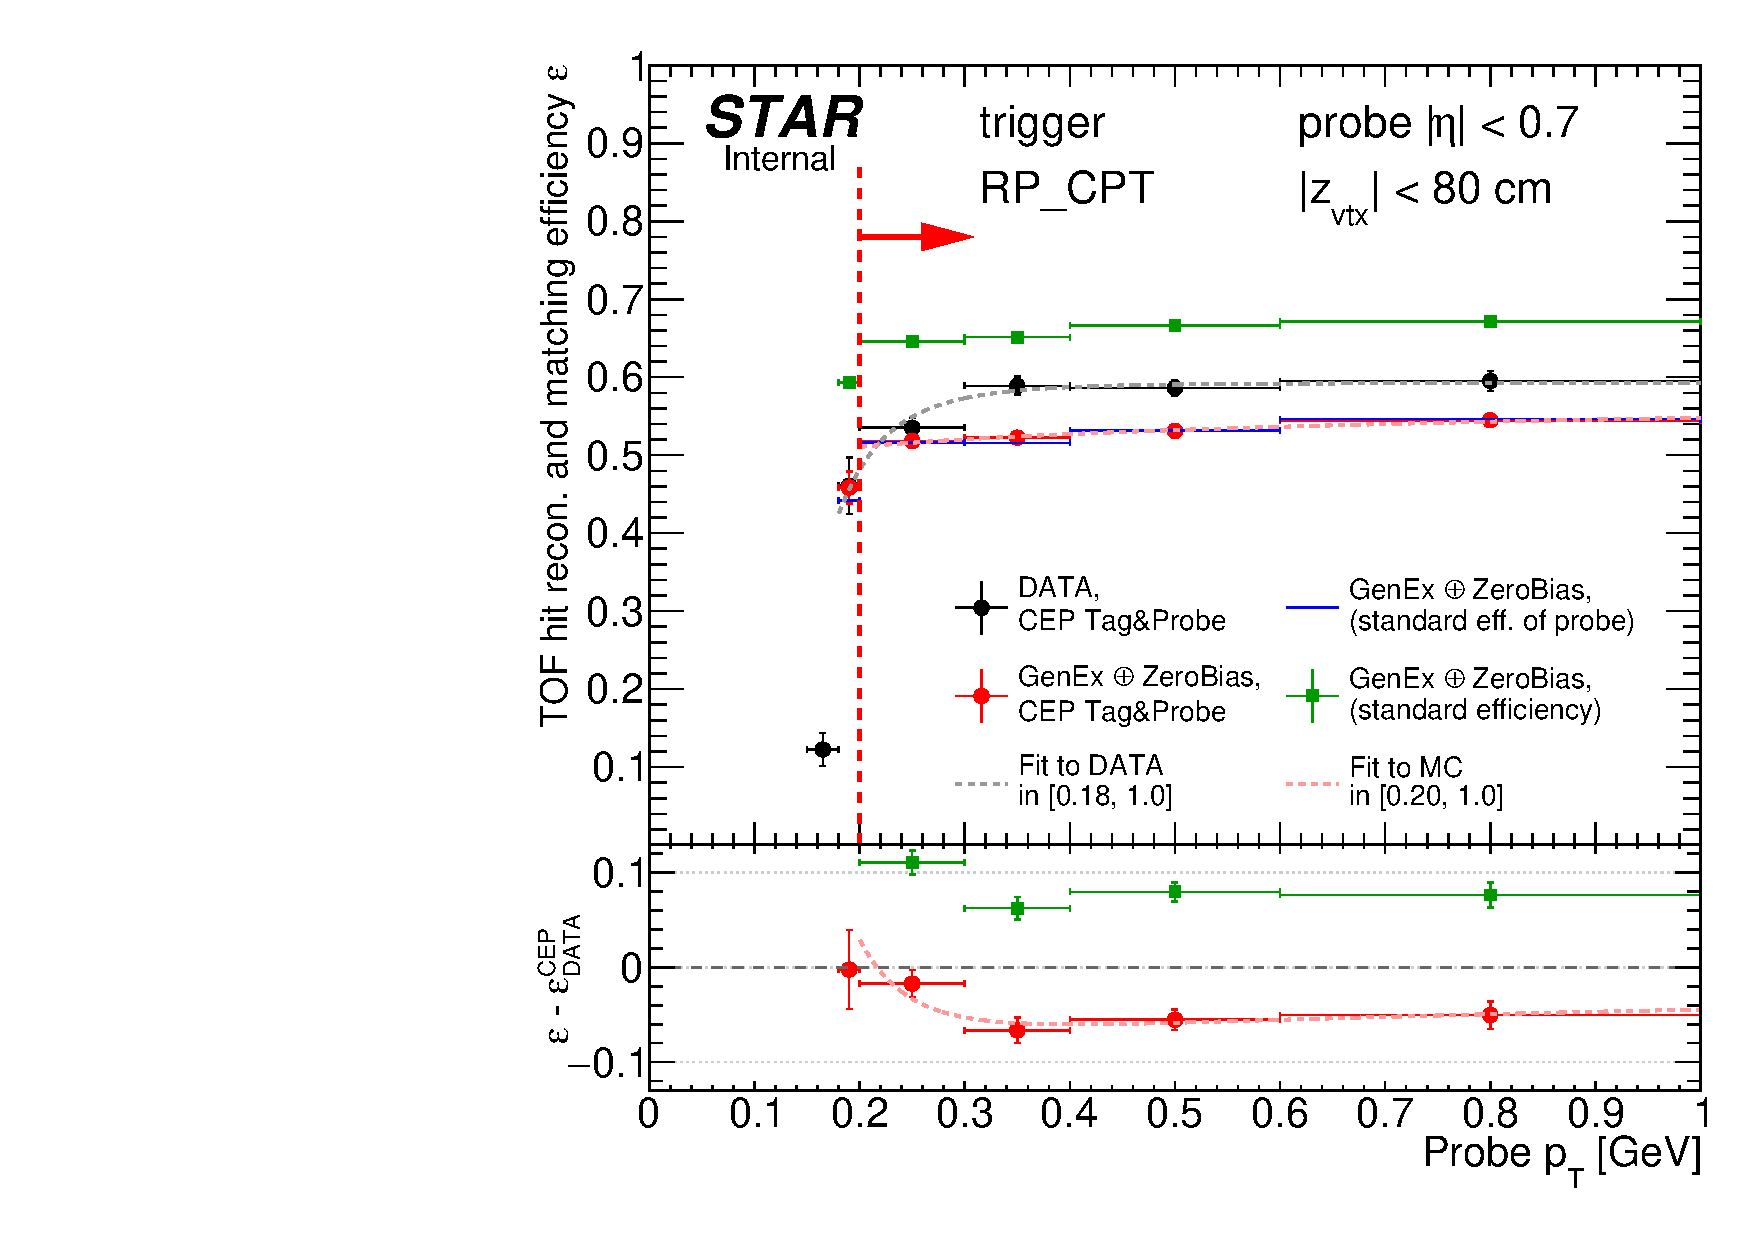
\includegraphics[width=\linewidth]{graphics/systematicsEfficiency/TOF_tagAndProbe/CPT/TofEffVsPt.pdf}\vspace{-5pt}}}
  \end{subfigure}
}
\quad
\parbox{0.4725\textwidth}{
  \centering
    \begin{subfigure}[b]{\linewidth}{
                \subcaptionbox{\label{fig:tofEffSystVsEta_CPT}}{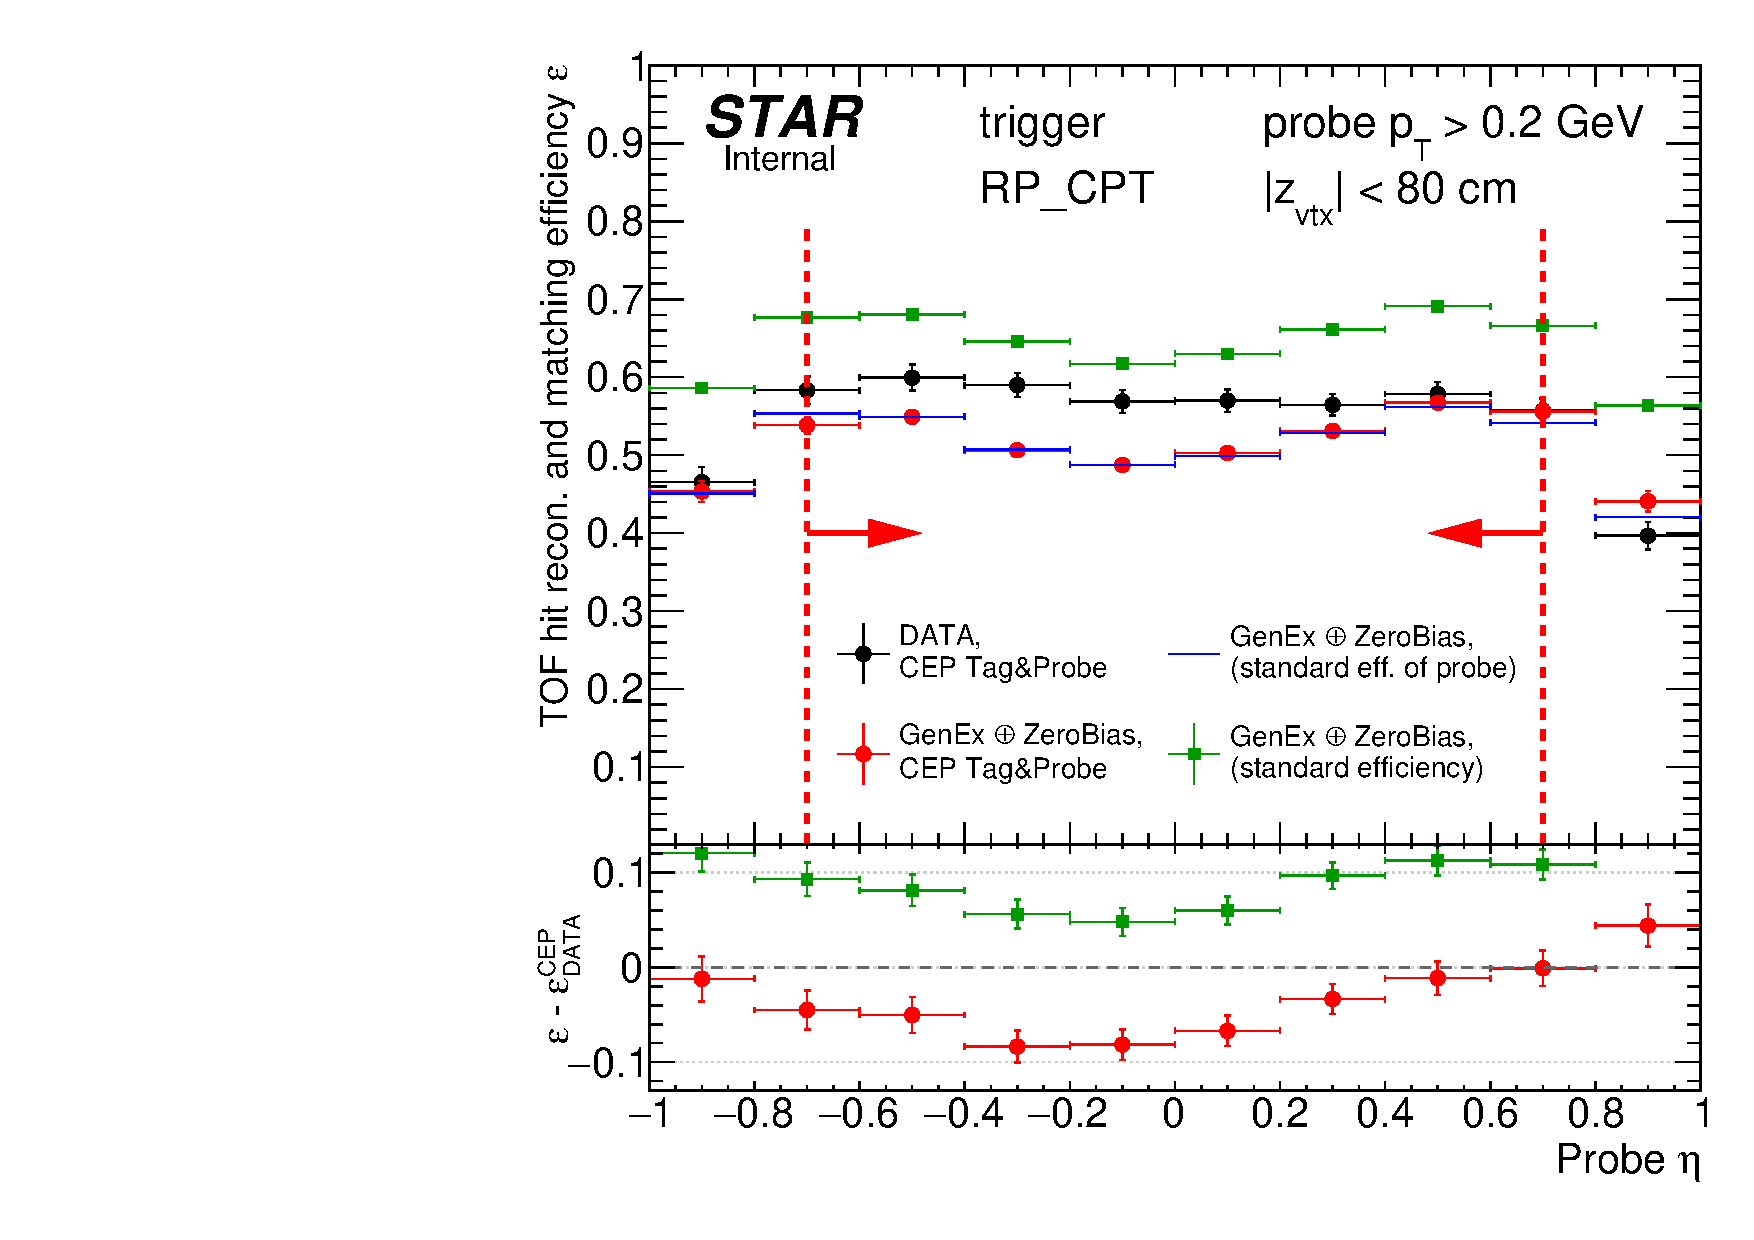
\includegraphics[width=\linewidth]{graphics/systematicsEfficiency/TOF_tagAndProbe/CPT/TofEffVsEta.pdf}\vspace{-5pt}}}
  \end{subfigure}
}%\vspace{-5pt}%
\caption[Tag\&Probe TOF efficiency from CEP data compared with the result from embedded CEP MC.]%
    {Tag\&Probe TOF efficiency from CEP data (black points) compared with the result from embedded CEP MC (red points) as a function of TPC track $p_{T}$ (top row) and $\eta$ (bottom row). The left and right hand side column represents results obtained from RP\_CPT and RP\_CPT2 triggers, respectively. Green points represent the TOF efficiency calculated in the standard way from embedded CEP MC sample. Blue lines denote the TOF efficiency calculated in the standard way solely from the selected probe tracks that were matched to primary pions at the true level. Difference between red points and blue lines show the potential bias of tag and probe method. Dashed lines are fits of function given by Eq.~\eqref{eq:tofEffFunc} to points of corresponding color. Dashed vertical lines with arrows indicate region of $p_{T}$ and $\eta$ accepted in analyses.}\label{fig:tofEffSyst}%
\end{figure}
%---------------------------


%---------------------------
\begin{figure}%[b!]%\vspace{-2pt}%
\centering%
\begin{minipage}{.4725\textwidth}%
  \centering%\vspace{11pt}
  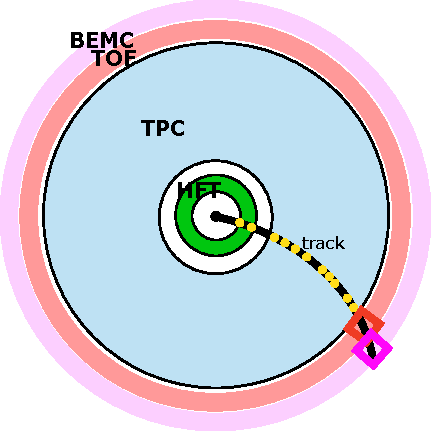
\includegraphics[width=0.965\linewidth]{graphics/systematicsEfficiency/TOF_tagAndProbe/effSketch.pdf}%\vspace{-5pt}%
  \caption[Sketch of the track with points in HFT.]%
  {Sketch of the cross section of the central detector and the track reconstructed with points in HFT. Presence of HFT points in a reconstructed track can be used as a tagger of the in-time tracks.}
  \label{fig:hftEffSketch}
\end{minipage}%
\quad\quad%
\begin{minipage}{.4725\textwidth}%
  \centering%
  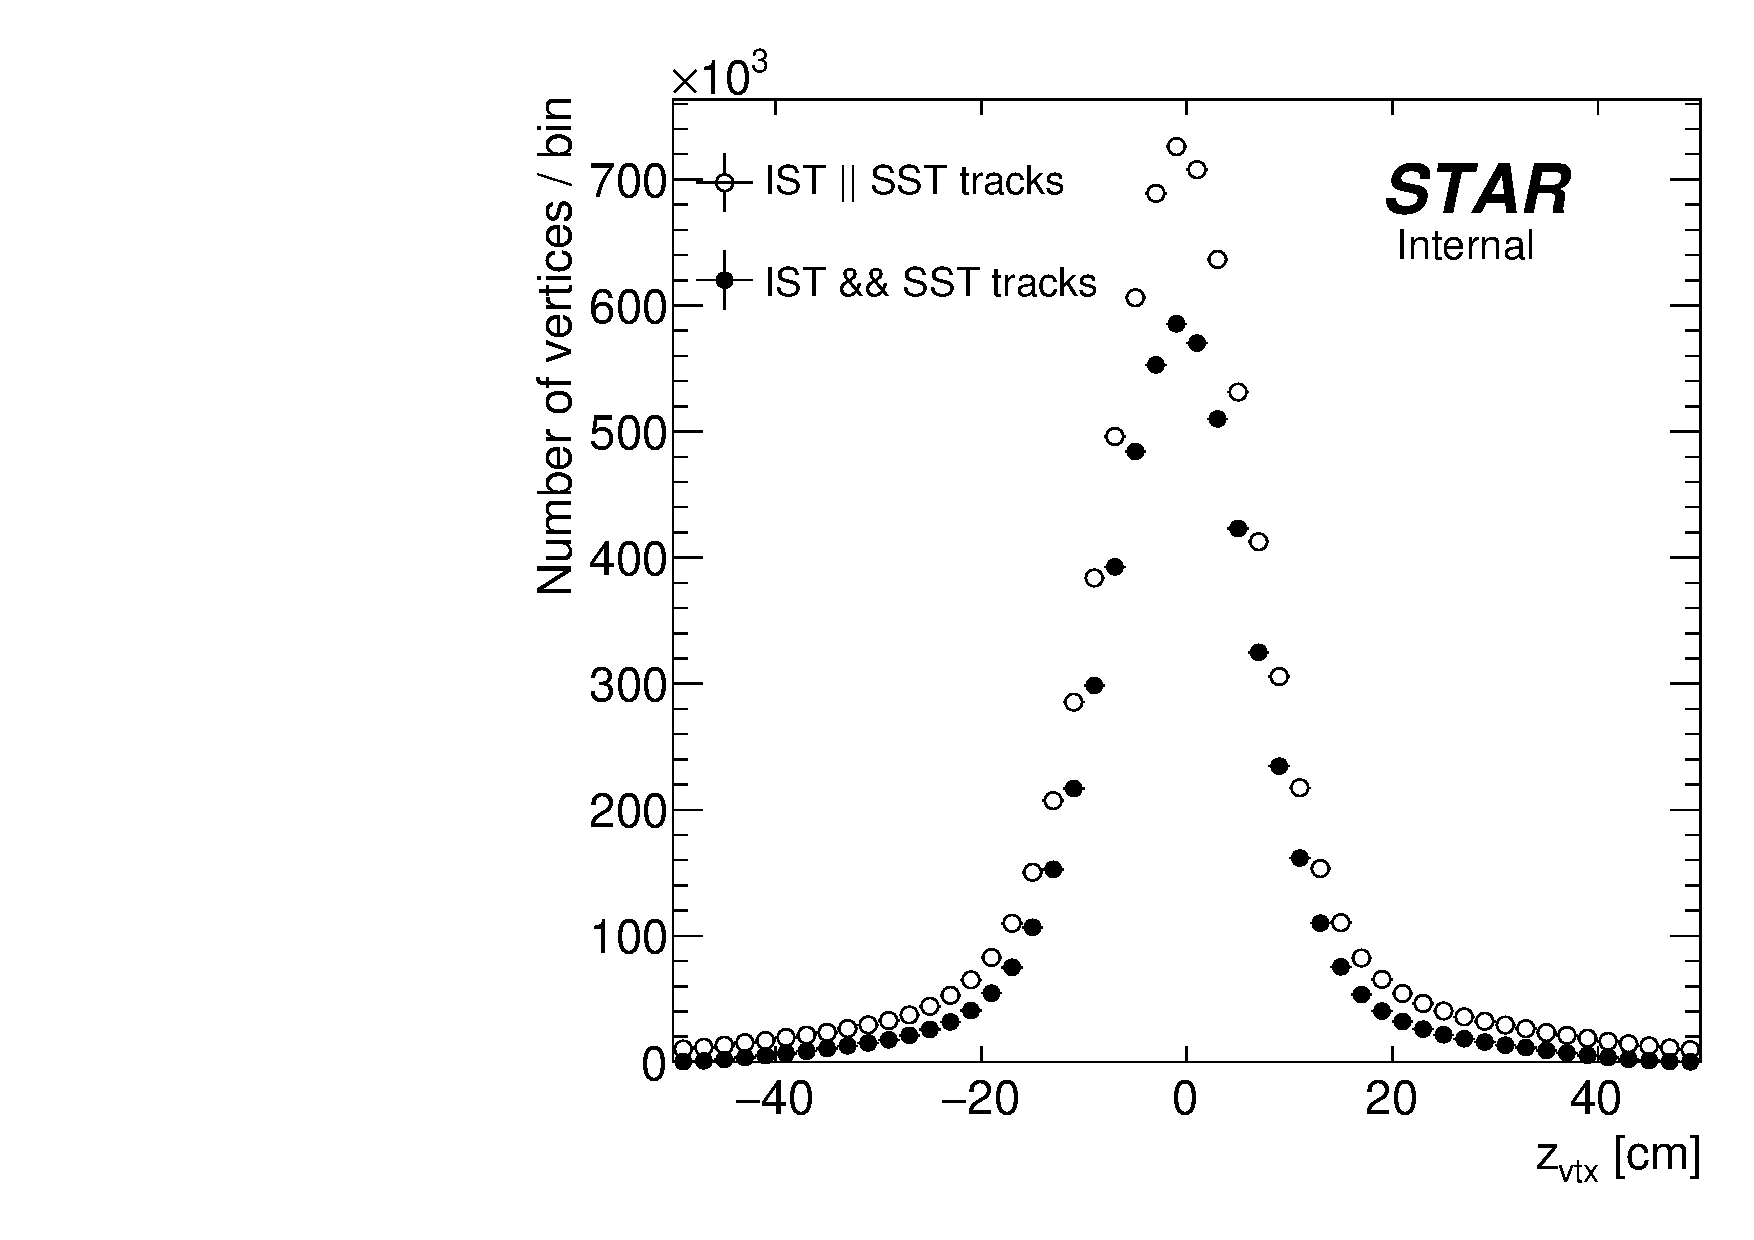
\includegraphics[width=\linewidth]{graphics/systematicsEfficiency/TOF_tagAndProbe/zVtxHFT.pdf}%\vspace*{-5pt}
  \caption[Distribution of $z$-position of vertices with TPC tracks containing hits in HFT.]
   {Distribution of $z$-position of vertices containing TPC tracks with HFT hits (st\_ssd stream). Open circles represent vertices with tracks with hits in IST or SST, full circles - IST and SST.}
   \label{fig:zVtxHFT}%\vspace*{-29pt}
\end{minipage}%
\end{figure}%
%---------------------------








% %---------------------------
% \begin{figure}[h!]
% \centering
% \parbox{0.4725\textwidth}{
%   \centering
%   \begin{subfigure}[b]{\linewidth}
%                 \subcaptionbox{\label{fig:tofEffSystVsPt}}{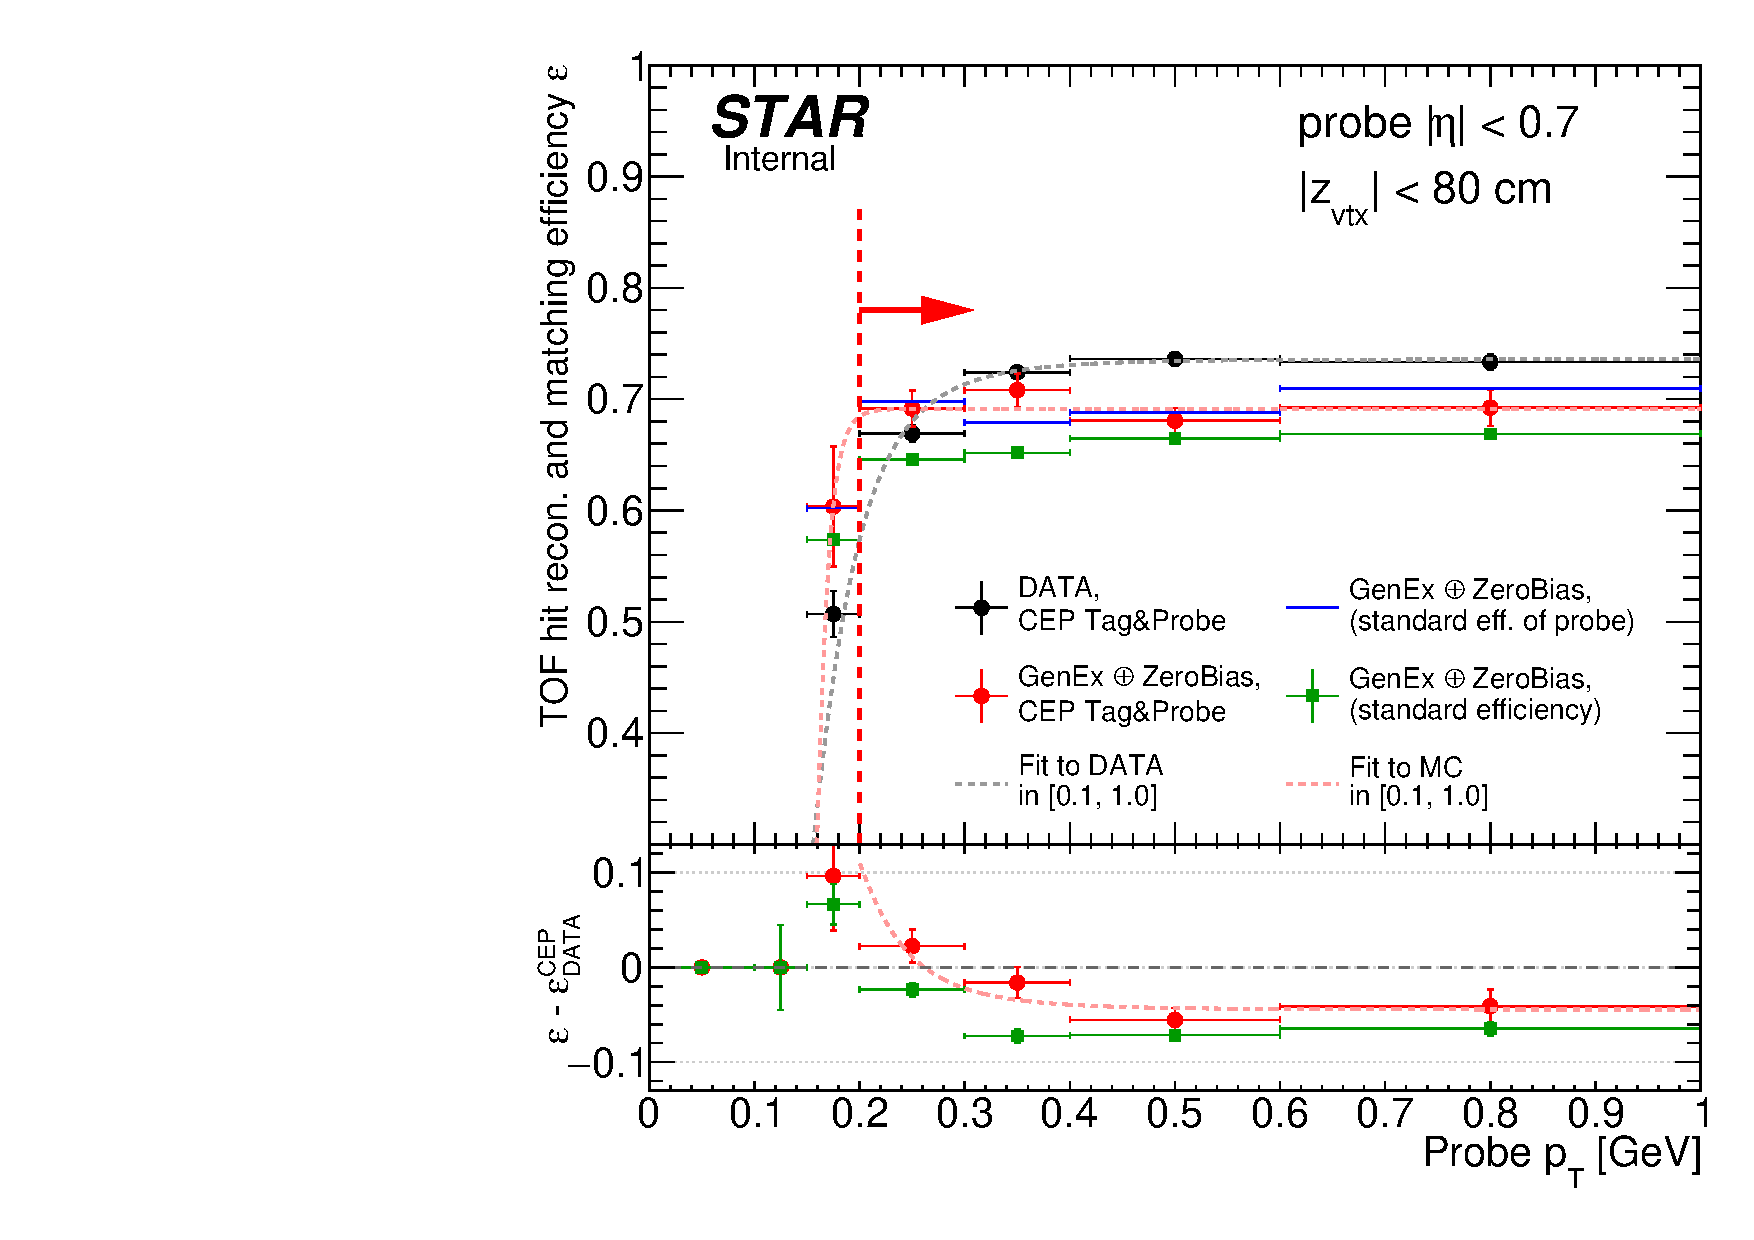
\includegraphics[width=\linewidth]{graphics/systematicsEfficiency/TOF_tagAndProbe/TofEffVsPt.pdf}}\vspace{-5pt}
%   \end{subfigure}
% }%
% \quad\quad%
% \parbox{0.4725\textwidth}{
%   \centering
%   \begin{subfigure}[b]{\linewidth}
%                 \subcaptionbox{\label{fig:tofEffSystVsEta}}{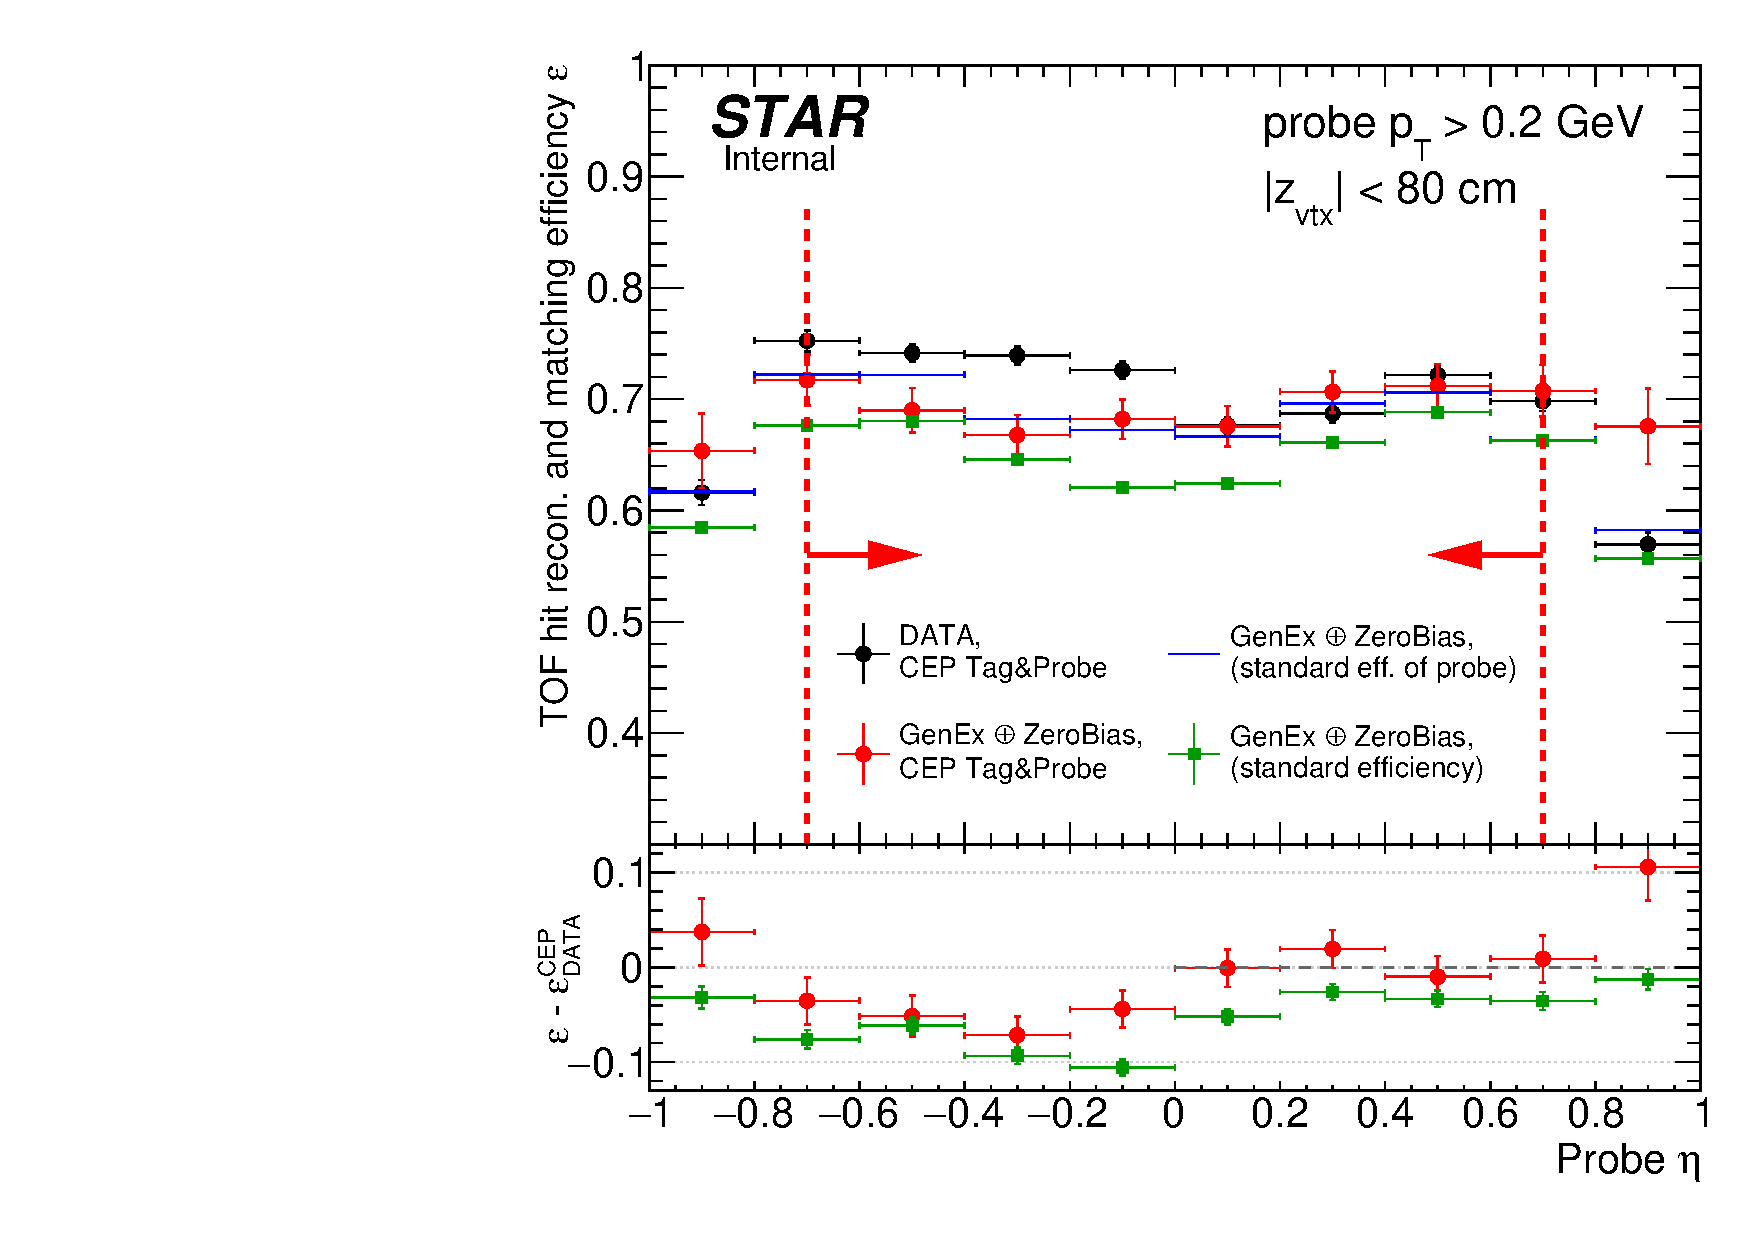
\includegraphics[width=\linewidth]{graphics/systematicsEfficiency/TOF_tagAndProbe/TofEffVsEta.pdf}}\vspace{-5pt}
%   \end{subfigure}
% }%
% \caption[Tag\&Probe TOF efficiency from CEP data compared with the result from embedded CEP MC.]%
%     {Tag\&Probe TOF efficiency from CEP data (black points) compared with the result from embedded CEP MC (red points) as a function of TPC track $p_{T}$ (\ref{fig:tofEffSystVsPt}) and $\eta$ (\ref{fig:tofEffSystVsEta}). Green points represent the TOF efficiency calculated in the standard way from embedded CEP MC sample. Blue lines denote the TOF efficiency calculated in the standard way solely from the selected probe tracks that were matched to primary pions at the true level. Difference between red points and blue lines show the potential bias of tag and probe method.}\label{fig:tofEffSyst}%
% \end{figure}
% %---------------------------



%---------------------------
\begin{figure}[h!]
\centering
\parbox{0.4725\textwidth}{
  \centering
  \begin{subfigure}[b]{\linewidth}{
                \subcaptionbox{\label{fig:tofEffSystVsPt_negativeEta_CPT}}{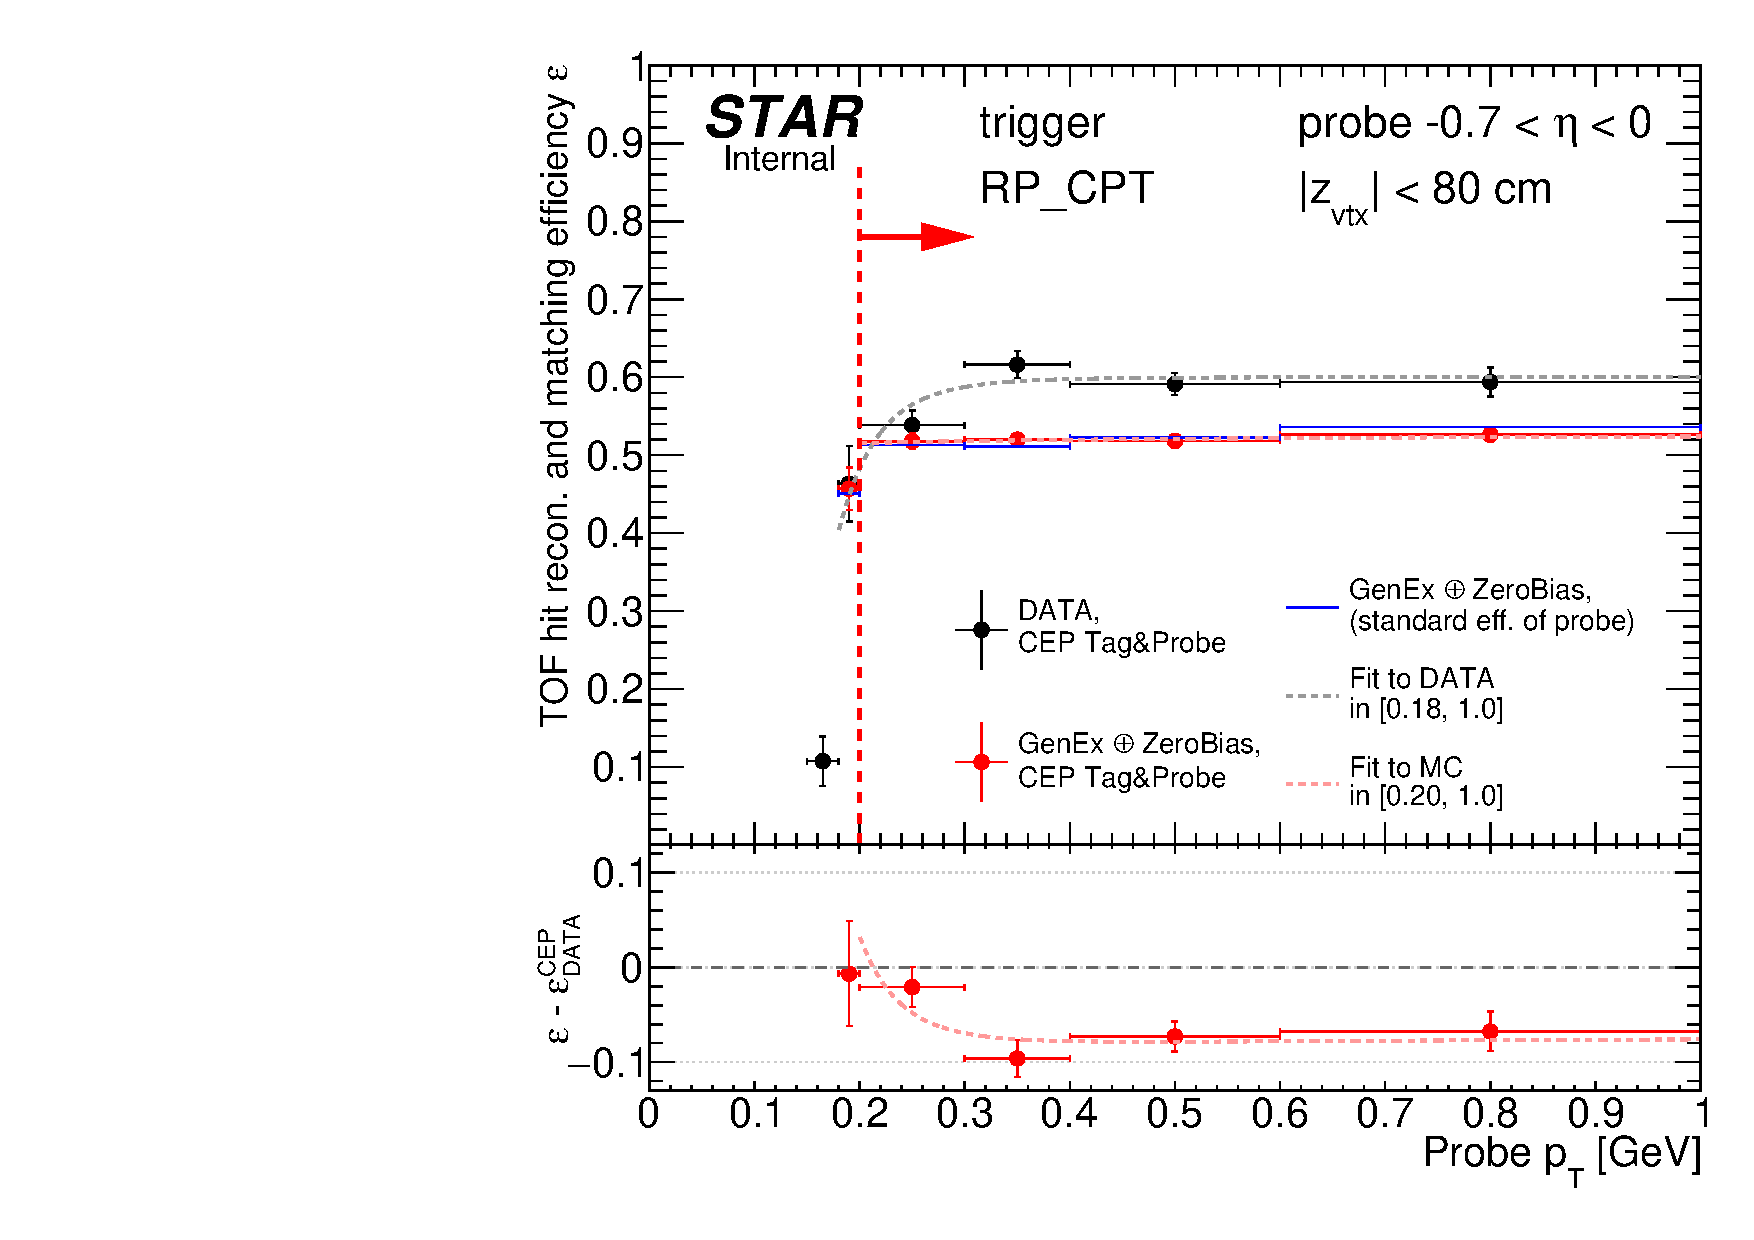
\includegraphics[width=\linewidth]{graphics/systematicsEfficiency/TOF_tagAndProbe/CPT/TofEffVsPt_negativeEta.pdf}\vspace{-5pt}}}
  \end{subfigure}\\[3pt]
  \begin{subfigure}[b]{\linewidth}\addtocounter{subfigure}{1}{
                \subcaptionbox{\label{fig:tofEffSystVsPt_positiveEta_CPT}}{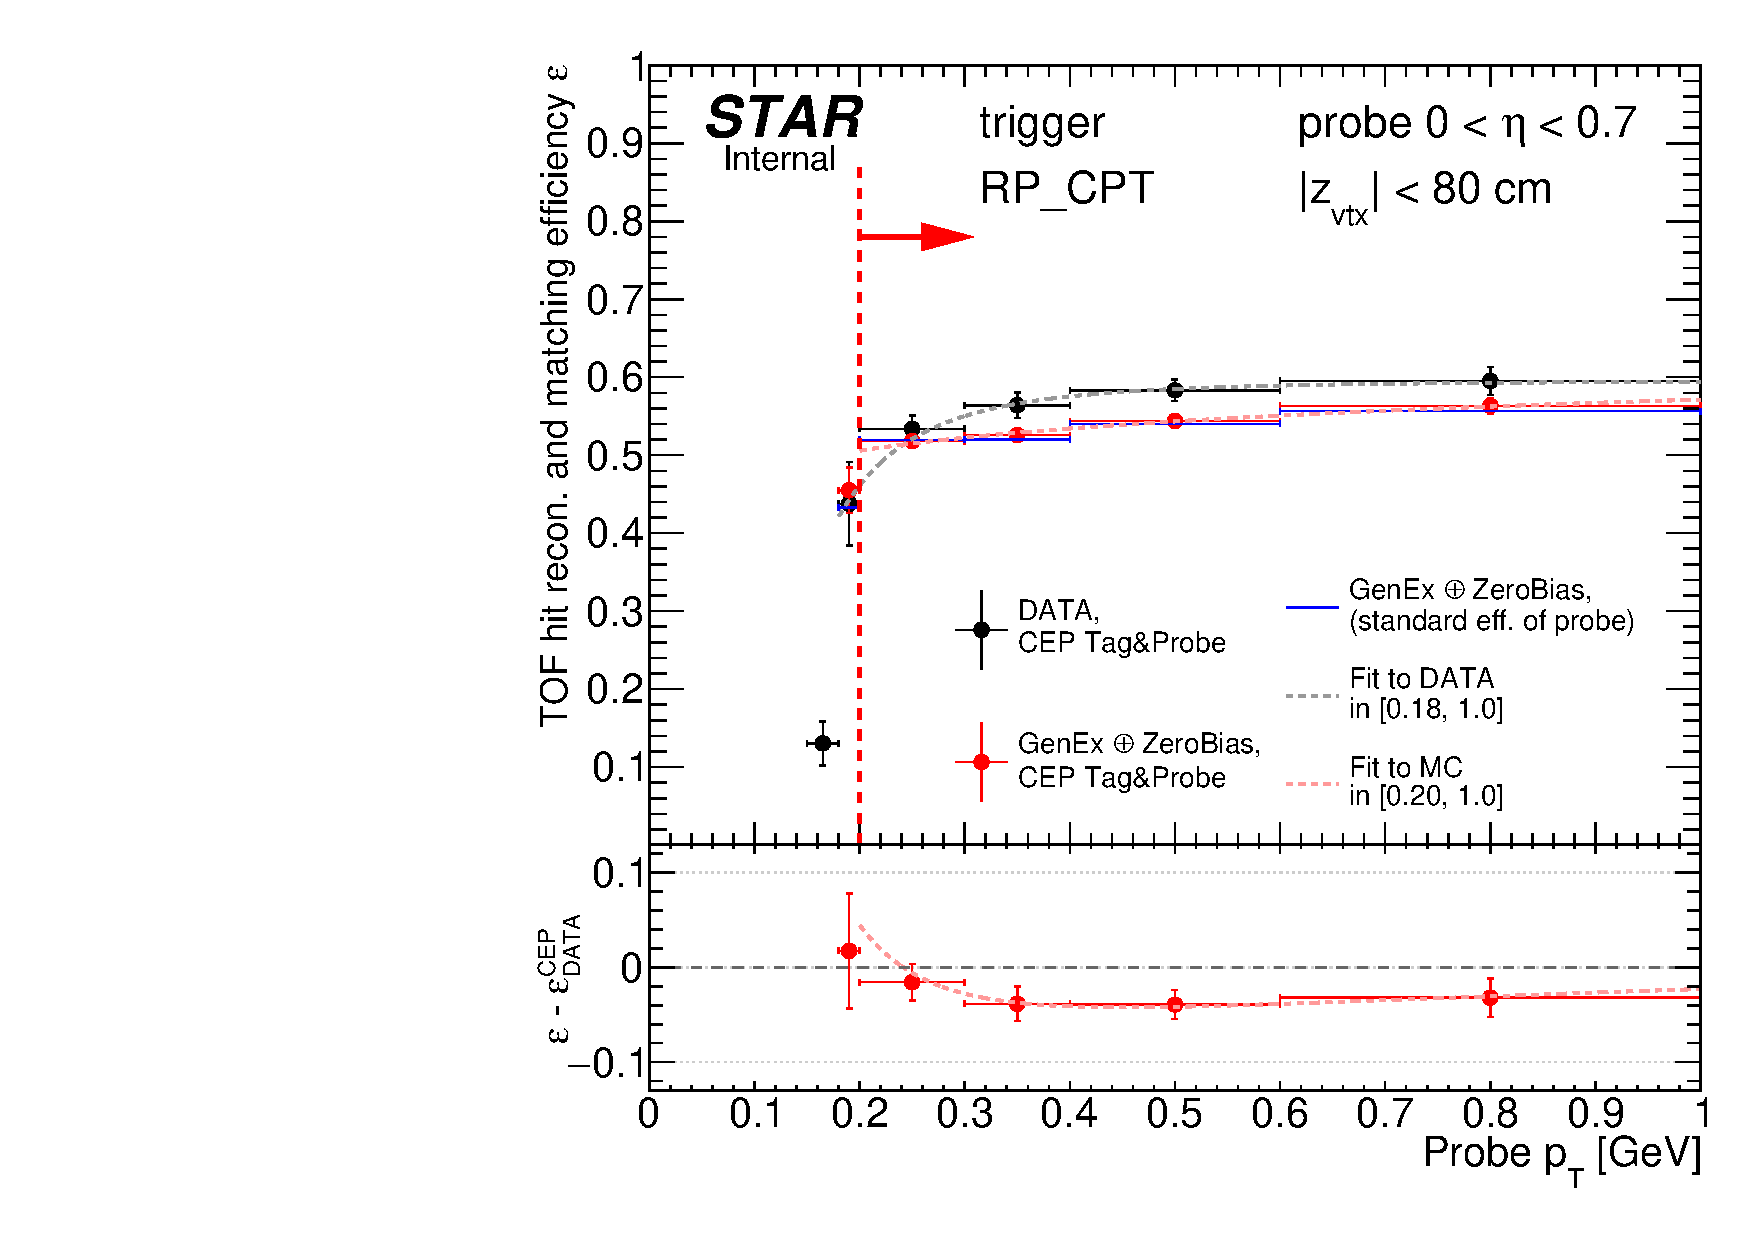
\includegraphics[width=\linewidth]{graphics/systematicsEfficiency/TOF_tagAndProbe/CPT/TofEffVsPt_positiveEta.pdf}\vspace{-5pt}}}
  \end{subfigure}
}
\quad
\parbox{0.4725\textwidth}{
  \centering
  \begin{subfigure}[b]{\linewidth}\addtocounter{subfigure}{-2}{
                \subcaptionbox{\label{fig:tofEffSystVsPt_negativeEta_CPT2}}{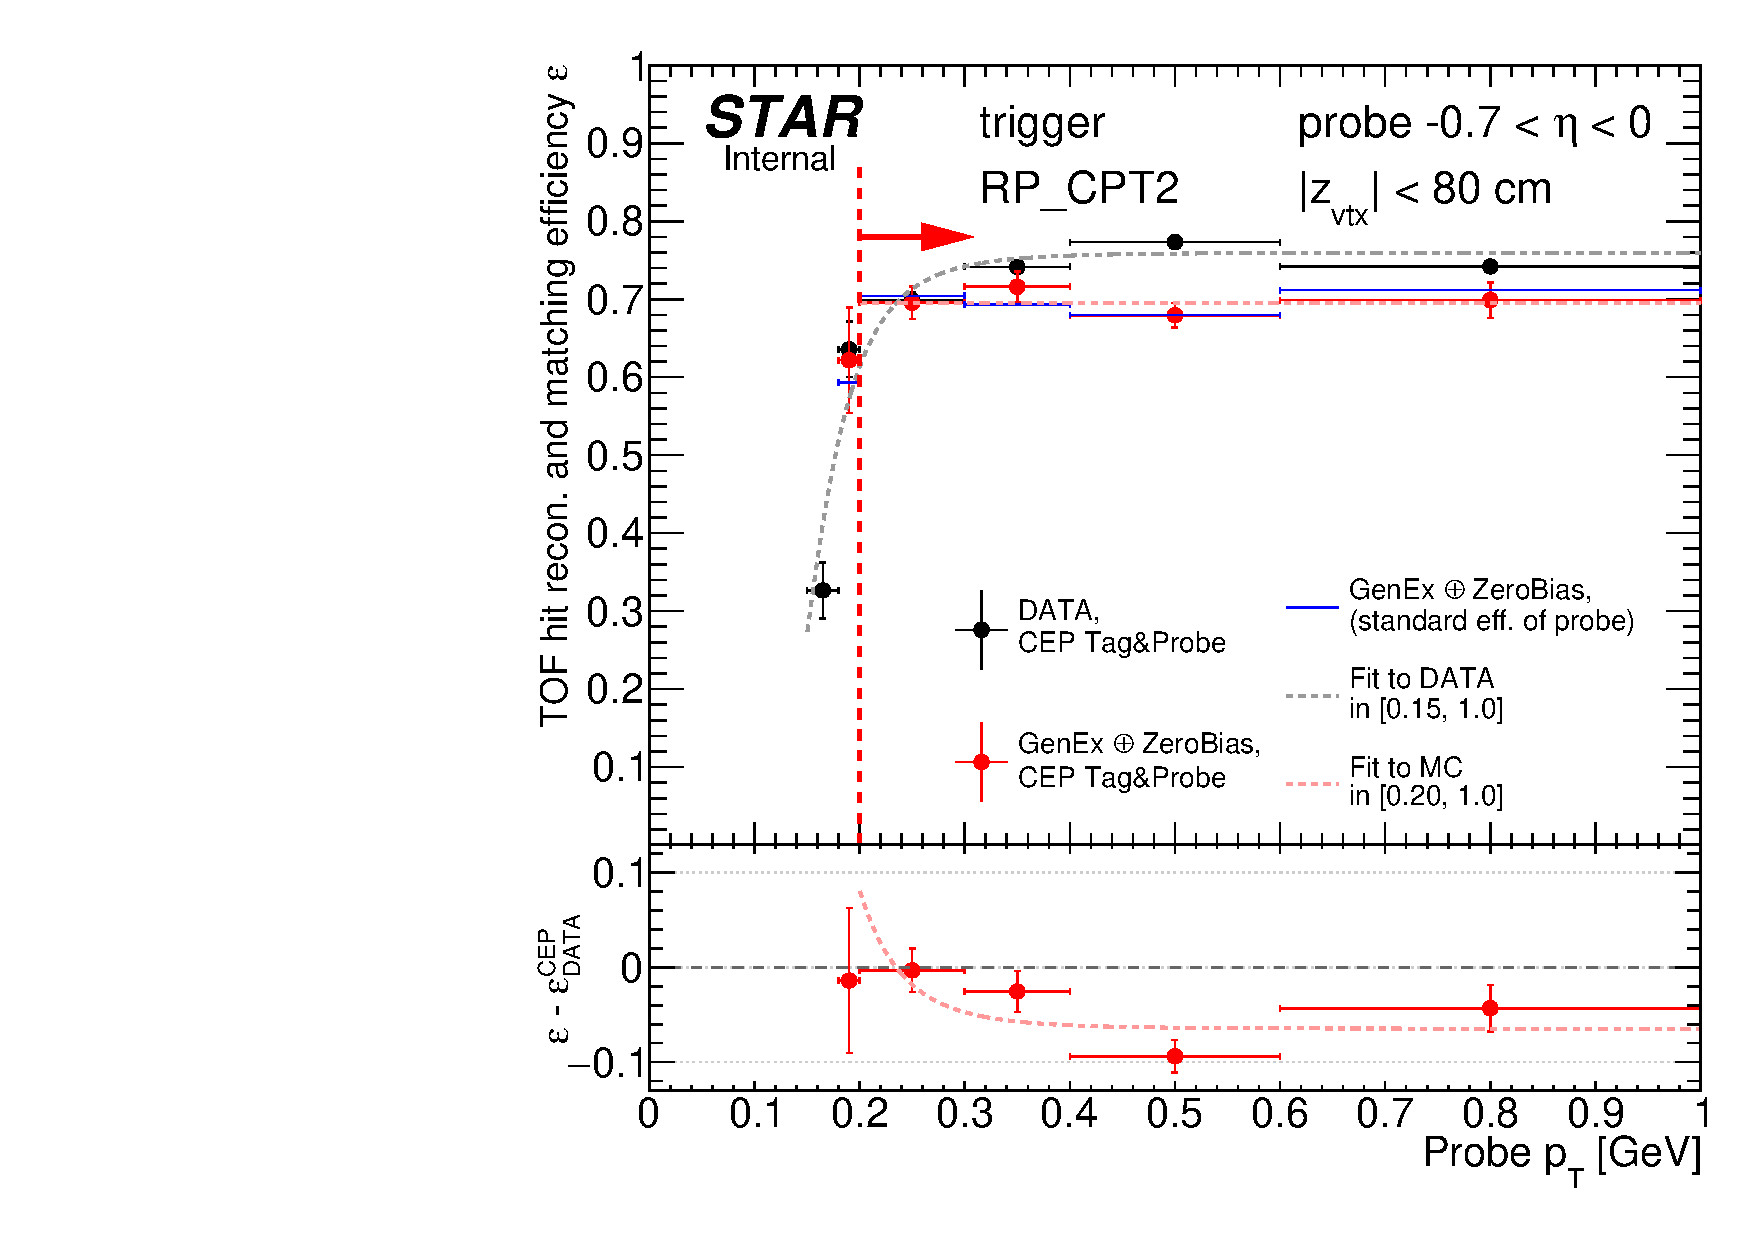
\includegraphics[width=\linewidth]{graphics/systematicsEfficiency/TOF_tagAndProbe/CPT2/TofEffVsPt_negativeEta.pdf}\vspace{-5pt}}}
  \end{subfigure}\\[3pt]
  \begin{subfigure}[b]{\linewidth}\addtocounter{subfigure}{1}{
                \subcaptionbox{\label{fig:tofEffSystVsPt_positiveEta_CPT2}}{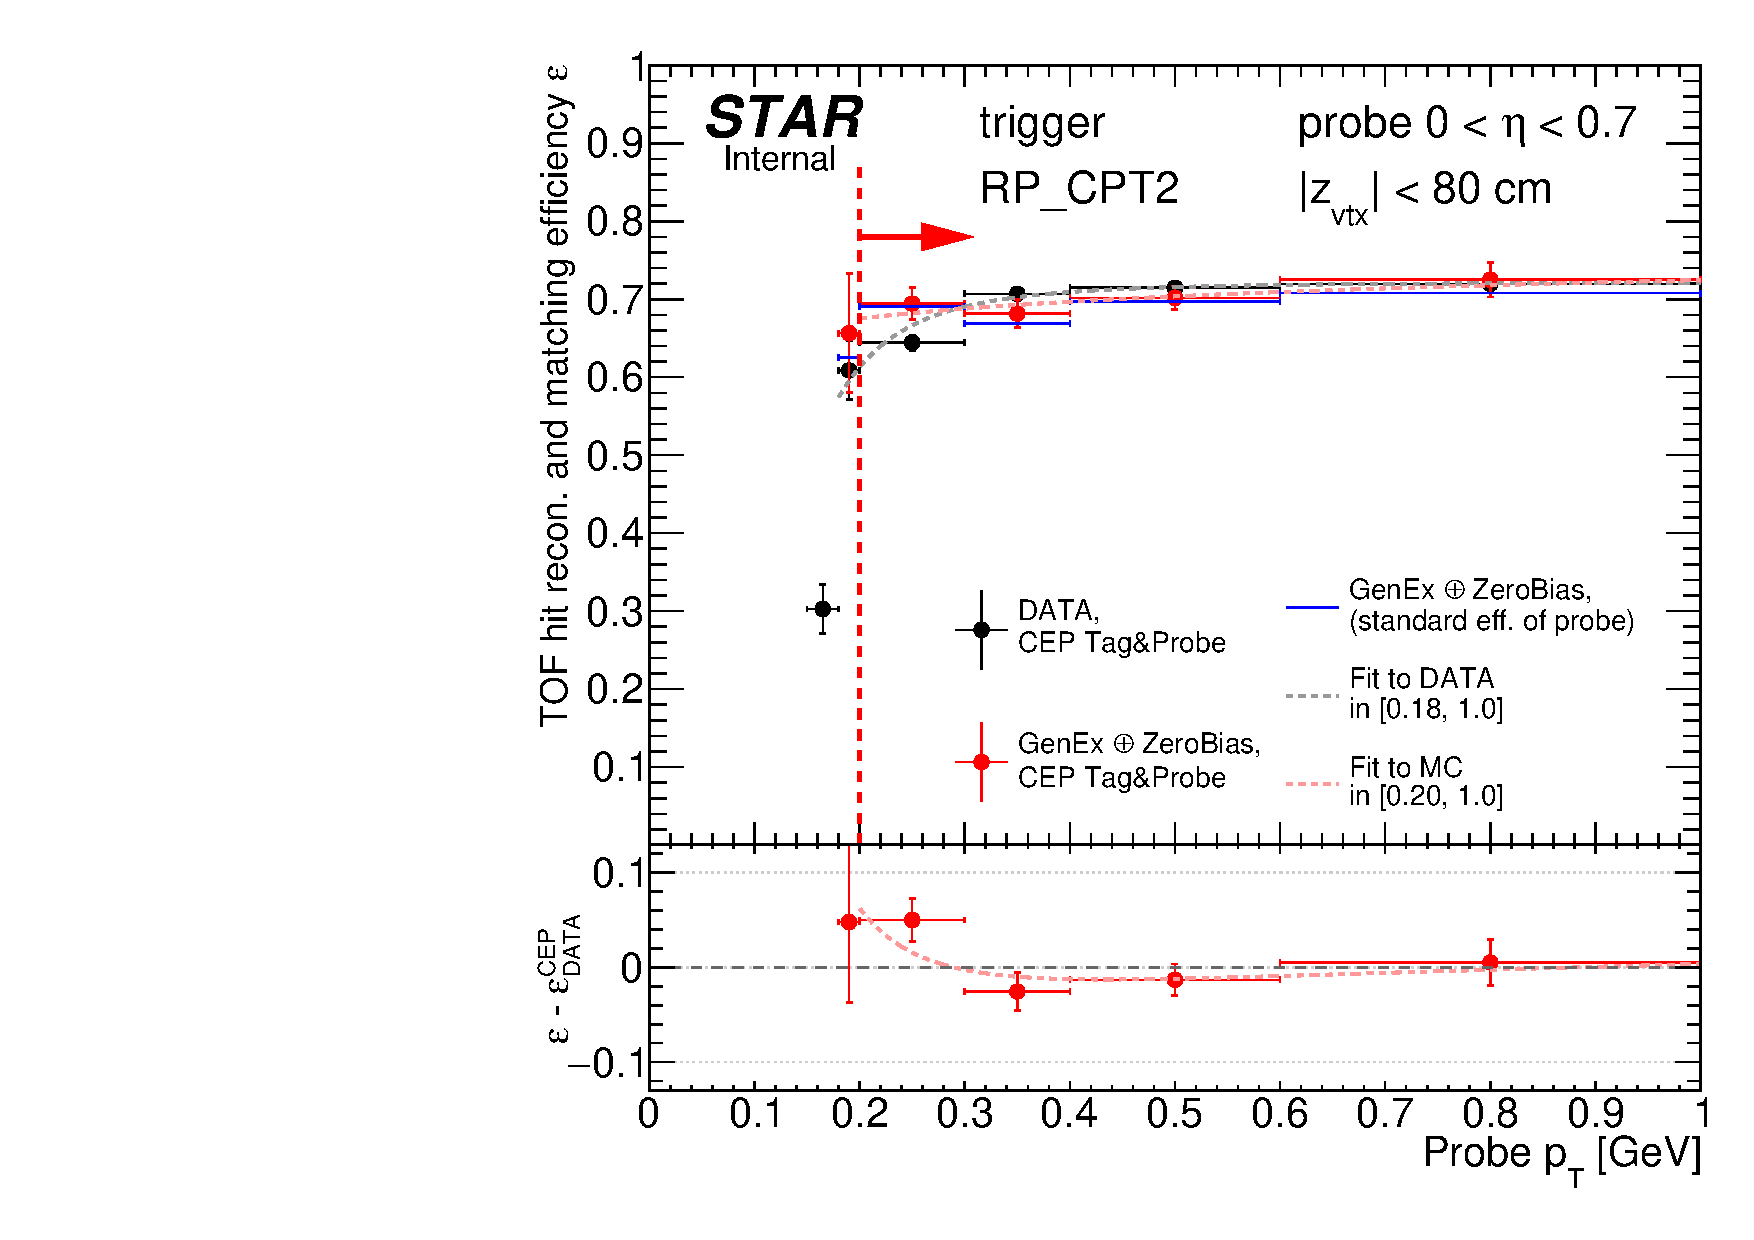
\includegraphics[width=\linewidth]{graphics/systematicsEfficiency/TOF_tagAndProbe/CPT2/TofEffVsPt_positiveEta.pdf}\vspace{-5pt}}}
  \end{subfigure}
}%\vspace{-5pt}%
\caption[Tag\&Probe TOF efficiency from CEP data compared with the result from embedded CEP MC (divided w.r.t. $\eta$ of the probe).]%
    {Tag\&Probe TOF efficiency from CEP data (black points) compared with the result from embedded CEP MC (red points) as a function of TPC track $p_{T}$ for negative (top row) and positive (bottom row) $\eta$ of the probe. The left and right hand side column represents results obtained from RP\_CPT and RP\_CPT2 triggers, respectively. Blue lines denote the TOF efficiency calculated in the standard way solely from the selected probe tracks that were matched to primary pions at the true level. Difference between red points and blue lines show the potential bias of tag and probe method. Dashed lines are fits of function given by Eq.~\eqref{eq:tofEffFunc} to points of corresponding color. Dashed vertical lines with arrows indicate region of $p_{T}$ and $\eta$ accepted in analyses.}\label{fig:tofEffSyst_etaBins}%
\end{figure}
%---------------------------
% %---------------------------
% \begin{figure}[h!]
% \centering
% \parbox{0.4725\textwidth}{
%   \centering
%   \begin{subfigure}[b]{\linewidth}
%                 \subcaptionbox{\label{fig:tofEffSystVsPt_negativeEta}}{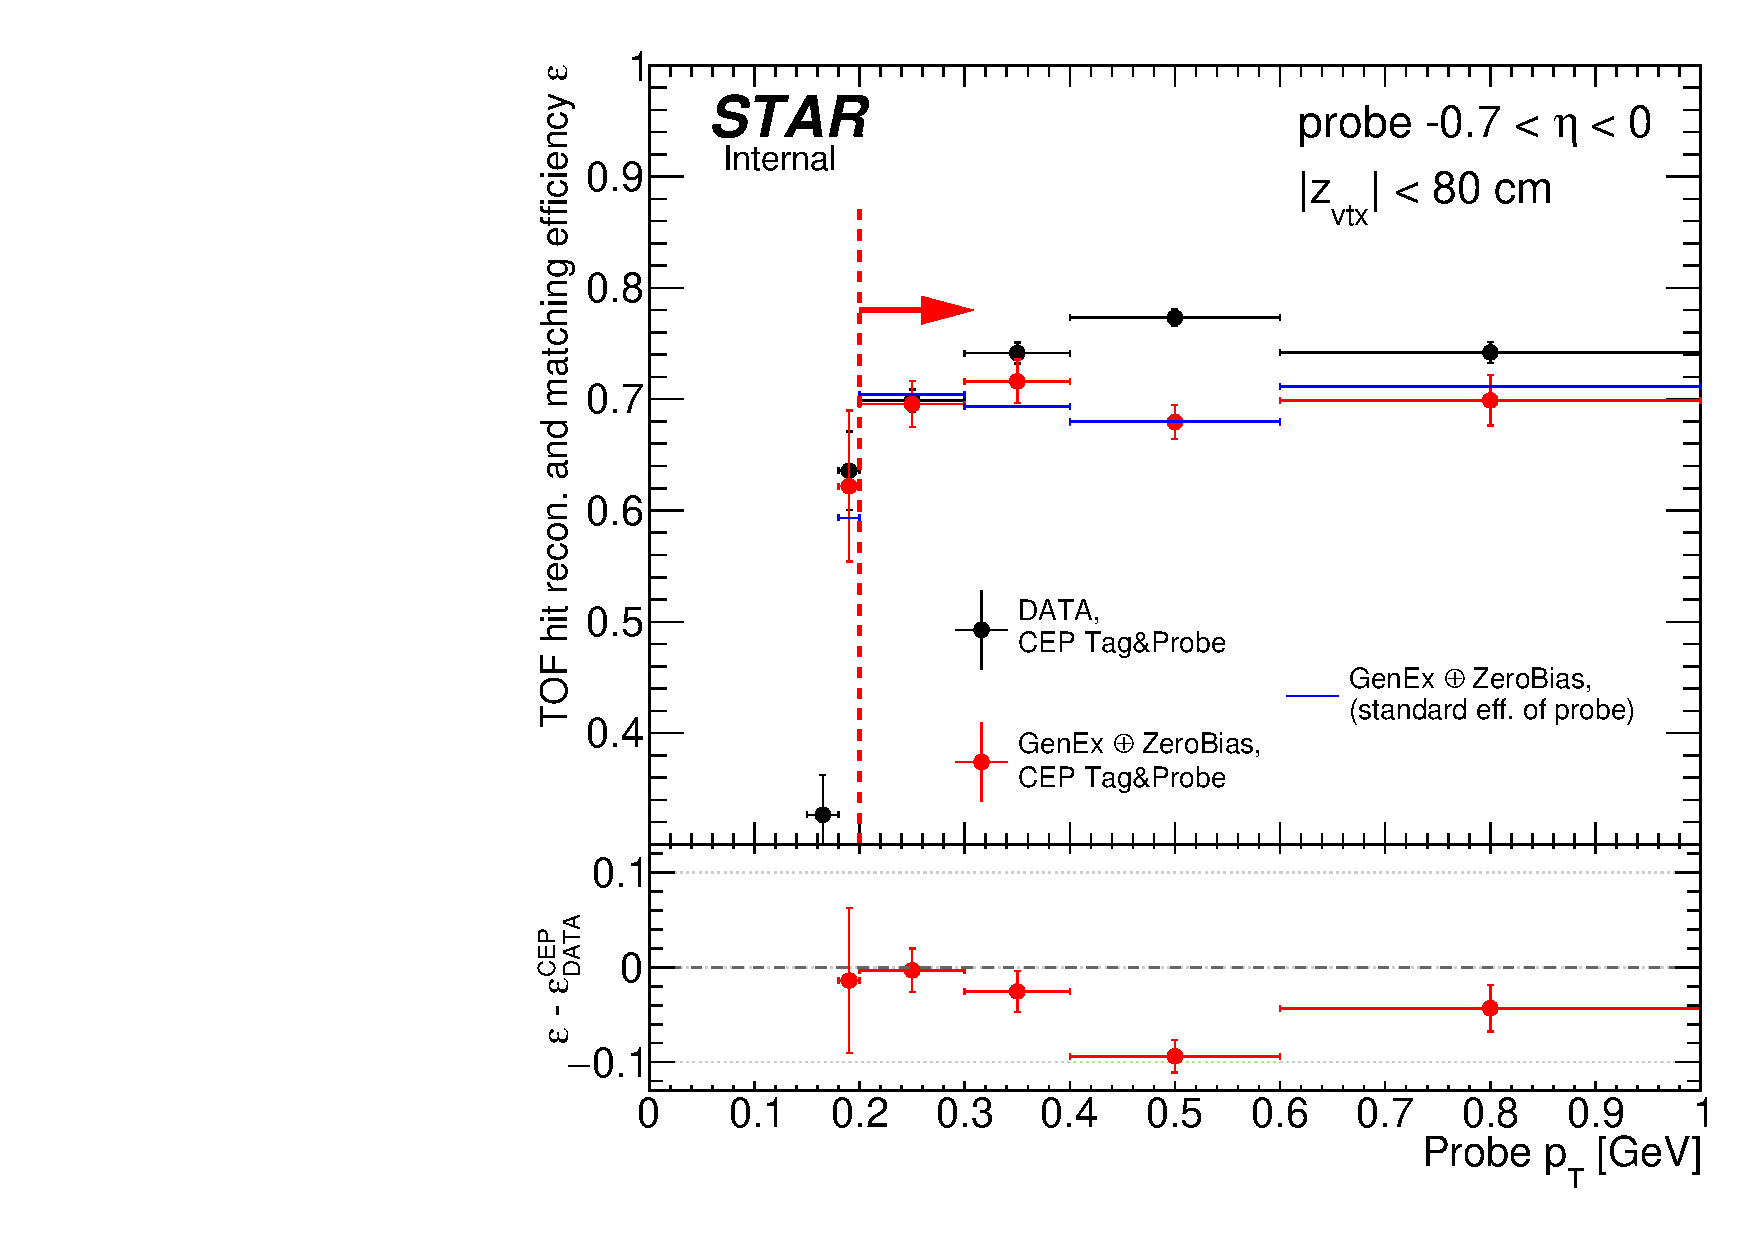
\includegraphics[width=\linewidth]{graphics/systematicsEfficiency/TOF_tagAndProbe/TofEffVsPt_negativeEta.pdf}}\vspace{-5pt}
%   \end{subfigure}
% }%
% \quad\quad%
% \parbox{0.4725\textwidth}{
%   \centering
%   \begin{subfigure}[b]{\linewidth}
%                 \subcaptionbox{\label{fig:tofEffSystVsPt_positiveEta}}{\includegraphics[width=\linewidth]{graphics/systematicsEfficiency/TOF_tagAndProbe/TofEffVsPt_positiveEta.pdf}}\vspace{-5pt}
%   \end{subfigure}
% }%
% \caption[ .]%
%     { .}\label{fig:tofEffSyst_etaBins}%
% \end{figure}
% %---------------------------